%!TEX TS-program = xelatex
%!TEX encoding = UTF-8 Unicode
\documentclass[a4paper, 12pt]{article}
\renewcommand{\baselinestretch}{1.5} 

%Notes:


%put in class[draft] to faster pre-compilation

\NeedsTeXFormat{LaTeX2e}
\usepackage{ifxetex}
\ifxetex
  \usepackage{fontspec}
  \usepackage{xltxtra}
  \usepackage[english]{babel}
\else
  \usepackage[utf8]{inputenc}
  \usepackage[english]{babel}
\fi
%\usepackage[slovak]{babel}
%\usepackage[czech]{babel}

\usepackage[super=false,usetitle=true]{achemso}
\bibpunct{[}{]}{,}{n}{}{;}
\def\citenumfont{\textrm}
\renewcommand\bibnumfmt[1]{#1. }
\def\pwidth{210}
\def\margin{25.0}
\hbadness=1350

\usepackage{titlesec}

\setcounter{secnumdepth}{4}

\titleformat{\paragraph}
{\normalfont\normalsize\bfseries}{\theparagraph}{1em}{}
\titlespacing*{\paragraph}
{0pt}{3.25ex plus 1ex minus .2ex}{1.5ex plus .2ex}


\usepackage{styles/bakalarska_prace}
\usepackage[top=3.0cm, bottom=3.0cm, left=3.5cm, right=2.5cm]{geometry}

%Extra packages
\usepackage{parskip}
\usepackage{amsmath}
\usepackage[flushleft]{threeparttable}
\usepackage{siunitx}
\usepackage{verbatim}
\usepackage{amssymb}  
\usepackage{graphicx}
\usepackage{multicol}
\usepackage{multirow}
\usepackage{physics}
\usepackage{bm}
\usepackage{nicefrac}
\usepackage{enumitem}
\usepackage[titletoc,title]{appendix}
%\usepackage{comment}
%\usepackage{cite}
%\usepackage{mciteplus}
\usepackage{tabu}
\usepackage{booktabs}
\usepackage{float}
\usepackage{subcaption}
\usepackage{mhchem}
\usepackage{xcolor}
\usepackage{listings}
\usepackage{pdfpages}
%dal experiment
\usepackage{caption}
\usepackage{subcaption}
%\usepackage{xkeyval}
\usepackage[export]{adjustbox}
\usepackage{graphicx}
%\usepackage{subfigure}
%\usepackage{underscore}
\mciteErrorOnUnknownfalse
\usepackage{natbib}
\setlength{\bibsep}{0.0pt}
\sisetup{output-exponent-marker=\ensuremath{\mathrm{e}}}
%\usepackage{wrapfig}

\newcommand{\kB}{k_{\text{B}}}
\newcommand{\rbold}{\mathbf{r}}
\newcommand{\angstrom}{\mbox{\normalfont\AA}}
\renewcommand{\thefootnote}{\fnsymbol{footnote}}

% %%%%%   LISTS   %%%%%%%%%%%%%%%%%%%%%
%deleting the headline of List of Figures
\makeatletter
\renewcommand\listoffigures{%
        \@starttoc{lof}%
}
%deleting the headline of List of Tables
\makeatletter
\renewcommand\listoftables{%
        \@starttoc{lot}%
}


% change Figure Caption
% \addto\captionsenglish{\renewcommand{\figurename}{Obrázek}}
% change TOC caption
% \addto\captionsenglish{\renewcommand{\contentsname}{Obsah}}
% change appendix caption
%\addto\captionsenglish{\renewcommand{\appendixname}{Příloha}}
% change Table Caption
%\addto\captionsenglish{\renewcommand{\tablename}{Tabulka}}


% %%%%%   MATLAB FORMAT   %%%%%%%%%%%%%%%%%%%%%
\definecolor{mygreen}{RGB}{28,172,0} 
\definecolor{mylilas}{RGB}{170,55,241}

\lstset{language=Matlab,%
    basicstyle=\ttfamily\small,
    breaklines=true,%
    morekeywords={matlab2tikz},
    keywordstyle=\color{black},%
    morekeywords=[2]{1}, keywordstyle=[2]{\color{black}},
    identifierstyle=\color{black},%
    stringstyle=\color{mylilas},
    commentstyle=\color{mygreen},%
    showstringspaces=false,%without this there will be a symbol in the places where there is a space
    numbers=left,%
    numberstyle={\tiny \color{black}},% size of the numbers
    numbersep=9pt, % this defines how far the numbers are from the text
    emph=[1]{for,end,break,function,if},emphstyle=[1]\color{blue}, %some words to emphasise
    %emph=[2]{word1,word2}, emphstyle=[2]{style},
    literate={á}{{\'a}}1
       {š}{{\v s}}1
       {č}{{\v c}}1
       {ž}{{\v z}}1
       {é}{{\'e}}1
       {í}{{\'i}}1
       {ý}{{\'y}}1
       {ú}{{\' u}}1
       {ľ}{{\v l}}1
       {ô}{{\^o}}1
       {ä}{{\"a}}1
       {ť}{{\v t}}1
       {ň}{{\v n}}1
}

% depth of 5 layers
% chapter,section,subsection,subsubsection,paragraph,subparagraph
\setcounter{secnumdepth}{5}
\setcounter{tocdepth}{5}

%equation counter according to sections
\numberwithin{equation}{section}


% %%%%%%%%%%%%%%%%%%%%%%%%%%%%%%%%%%%%%%%%%%%%%%%%%%%%%%%%%%%%%%%%%%%%%%%%%
% %%%%%%%%%%%%%%%%%%%%%%%%%%%%%%%%%%%%%%%%%%%%%%%%%%%%%%%%%%%%%%%%%%%%%%%%%
% %%%%%%%%%%%%%%%%%%%%%%%%%%%%%%%%%%%%%%%%%%%%%%%%%%%%%%%%%%%%%%%%%%%%%%%%%
% %%%%%%%%%%%%%%%%%%%%%%%%%%%%%%%%%%%%%%%%%%%%%%%%%%%%%%%%%%%%%%%%%%%%%%%%%
% %%%%%%%%%%%%%%%%%%%%%%%%%%%%%%%%%%%%%%%%%%%%%%%%%%%%%%%%%%%%%%%%%%%%%%%%%
% %%%%%%%%%%%%%%%%%%%%%%%%%%%%%%%%%%%%%%%%%%%%%%%%%%%%%%%%%%%%%%%%%%%%%%%%%

\begin{document}
\thispagestyle{empty}
% %%%%%%%%%%%%%%%%%%%%%%%%%%%%%%%%%%%%%%%%%%%%%%%%%%%%%%%%%%%%%%%%%%%%%%%%%
% ACKNOWLEDGEMENT, SUMMARY, Contents
%%%%%%%%%%%%%%%%%%%%%%%%%%%%%%%%%%%%%%%%%%%%%%%%%%%%%%%%%%%%%%%%%%%%%%%%
% FRONTPAGE
%\newpage
%
\includepdf[pages={1}]{documents/frontpage_placeholder.pdf} 
%replace your document

%%%%%%%%%%%%%%%%%%%%%%%%%%%%%%%%%%%%%%%%%%%%%%%%%%%%%%%%%%%%%%%%%%%%%%%%
% ASSIGNMENT
%\newpage
%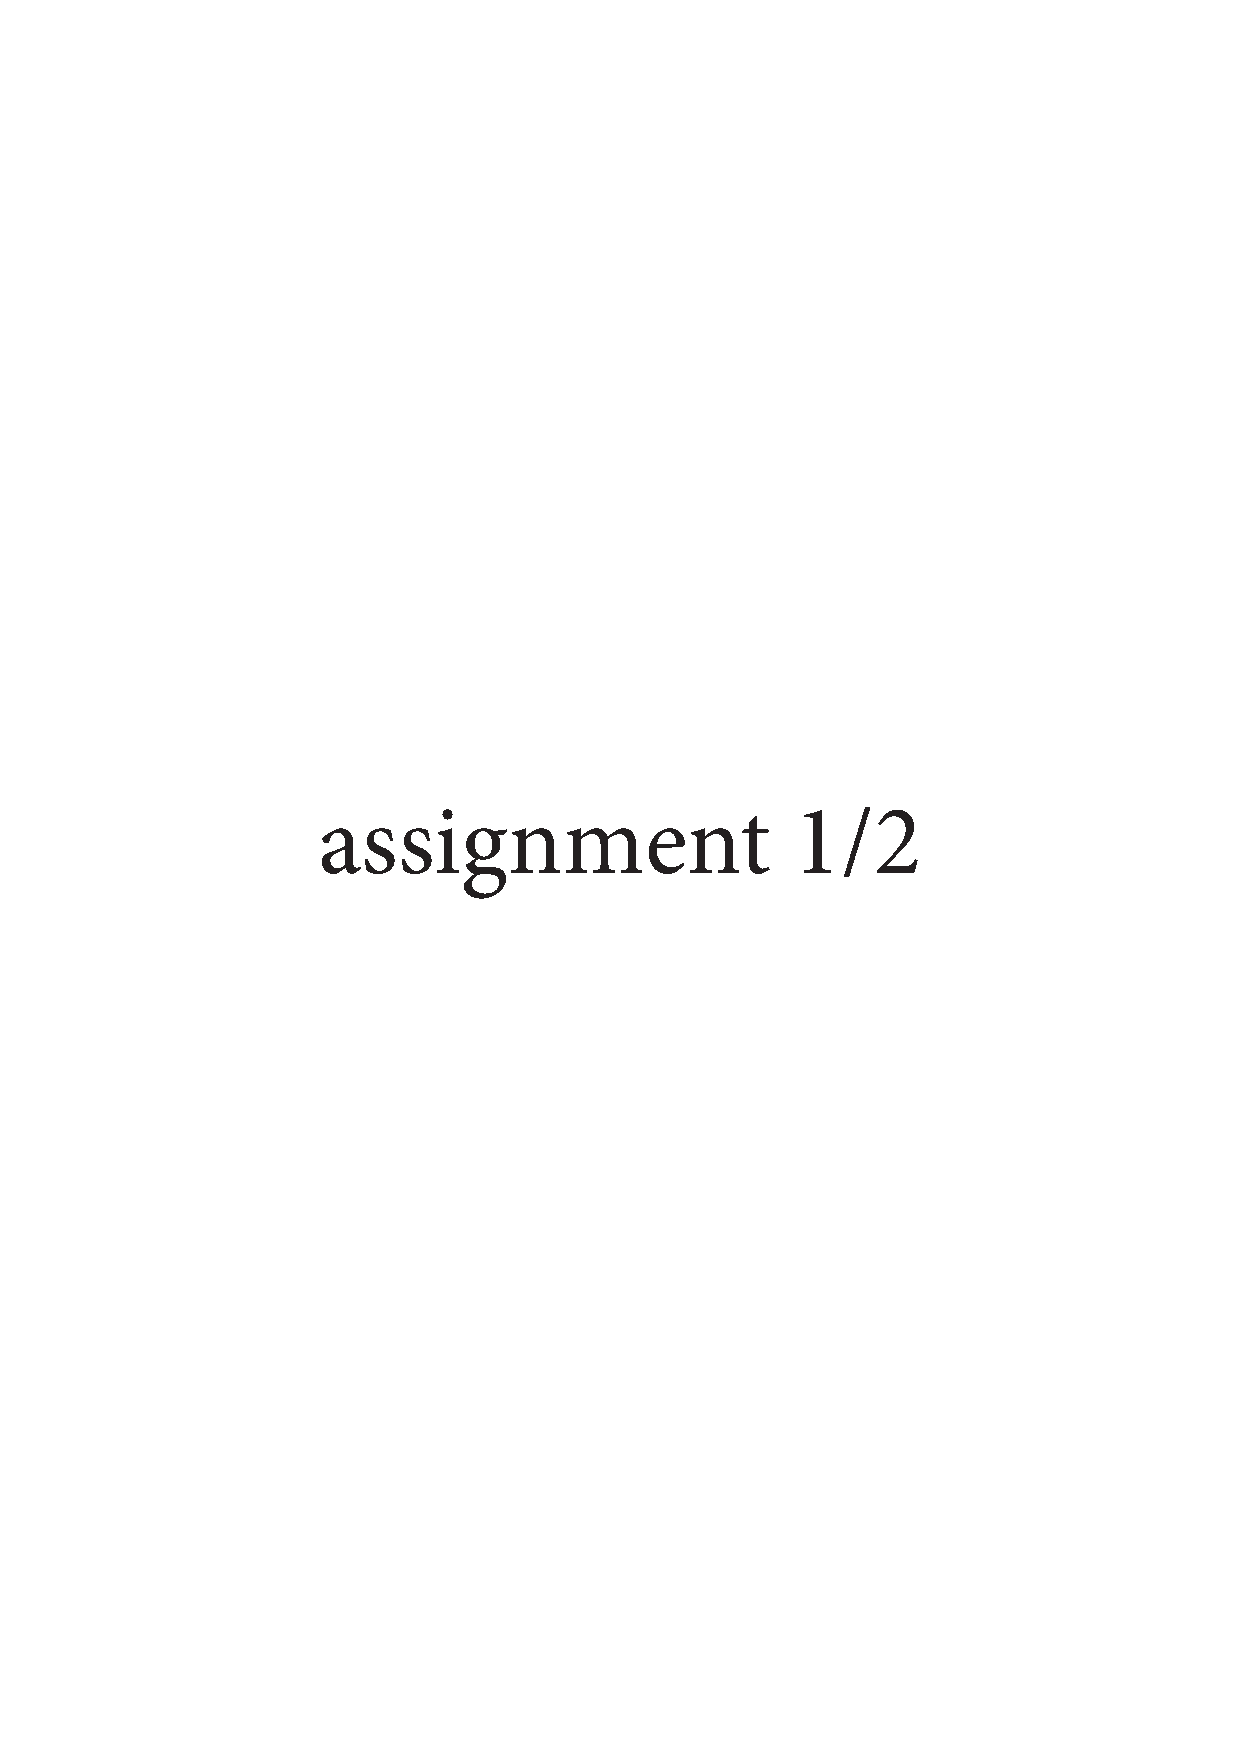
\includepdf[pages={1,2}]{documents/assignment_placeholder.pdf}
%replace your document

%%%%%%%%%%%%%%%%%%%%%%%%%%%%%%%%%%%%%%%%%%%%%%%%%%%%%%%%%%%%%%%%%%%%%%%%
% ACKNOWLEDGEMENT

\newpage
\thispagestyle{empty}

\vspace*{\fill}
\section*{ACKNOWLEDGEMENT}
\mbox
\indent First and foremost, I would like to express my sincere gratitude to my supervisor, Assoc. Prof. Ing. Ctirad Červinka, Ph.D. for his valuable advice on my way of learning the tools of computational chemistry, the opportunity to participate in real research and for the time devoted during consultations. Special thanks also go to my consultant Ing. Jan Ludík and lab fellow Ing. Petr Touš, for their expert advice and help during the results analysis and solving the simulation errors. Computational resources were provided by the e-INFRA CZ project (ID:90254), supported by the Ministry of Education, Youth and Sports of the Czech Republic.

%\vspace*{\fill}
% \noindent Práce byla podpořena projekty Grantové agentury ČR č. ...


%%%%%%%%%%%%%%%%%%%%%%%%%%%%%%%%%%%%%%%%%%%%%%%%%%%%%%%%%%%%%%%%%%%%%%%%

% SUMMARY

\newpage
\thispagestyle{empty}

\section*{SUMMARY}
Limited bioavailability of numerous active pharmaceutical ingredients is due to the poor solubility of their crystalline phases in water. The preparation of amorphous solid dispersions with biocompatible polymers offer a solution to overcome this problem, which currently limits the wider use of many drugs. This work presents a solution in the form of molecular dynamic modelling of binary systems composed of selected poorly soluble active pharmaceutical ingredients and polylactic acid as a representative of biocompatible polymer excipient. Molecular dynamics tools are used to investigate the structural and cohesive properties of pure compounds and their mixtures, with special emphasis on the analysis of molecular interactions and compatibility between drug and excipient molecules. Different simulation setups for full atomic resolution polymer simulations are validated and compared with existing experimental data, in particular glass transition temperatures and densities.

The glass transition temperature indicate the influence of atomic interactions between the drug and polymer molecules forming a more favorable amorphous binary mixture. For three of the four active pharmaceutical ingredients studied, we find that mixing them with a polylactic acid results in the formation of a more favorable amorphous binary mixture. These substances showed the highest degree of polymer-drug interactions. The development of reliable computational models evaluating drug interactions with polymeric excipients will contribute to the rational design of new drug formulations in the future.


\subsection*{keywords:}
\textit{Active pharmaceutical ingredients, Biocompatible polymer excipients, Amorphous solid dispersions, Glass transitions, Molecular dynamics}

%\bigskip %space between paragraphs
\newpage
\thispagestyle{empty}
\section*{SOUHRN}
Omezená biologická dostupnost mnoha aktivních farmaceutických látek se objevuje v důsledku špatné rozpustnosti jejich krystalických fází ve vodě. Příprava amorfních disperzí léčiv s biokompatibilními polymery nabízejí řešení k překonání tohoto problému, který v současnosti omezuje širší používání mnoha léčiv. Tato práce předkládá řešení v podobě molekulárně-dynamického modelování binárních systémů obsahujících vybrané špatně rozpustné účinné farmaceutické složky a kyselinu polymléčnou jako zástupce biokompatibilních polymerních excipientů. Nástroje molekulové dynamiky jsou použity ke zkoumání strukturních a kohezních vlastností čistých látek i jejich směsí se zvláštním důrazem na analýzu molekulárních interakcí a kompatibility mezi molekulami léčiva a pomocné látky. Ověřena jsou různá simulační nastavení pro simulace polymeru v plném atomovém rozlišení a srovnána s existujícími experimentálními daty, zejména teploty skelného přechodu a hustoty.

Na teplotě skelného přechodu se ukazuje, že míra vzájemných atomových interakcí mezi molekuly léčiva a polymeru ovlivňuje formování výhodnější amorfní binární směsi. Pro tři ze čtyř studovaných farmaceuticky aktivních látek zjišťujeme, že jejich mísením s polymléčnou kyselinou dochází k formaci výhodnější amorfní binární směsi. Tyto látky vykazovaly největší míru interakcí mezi polymerem a léčivem. Vývoj spolehlivých výpočetních modelů hodnotících interakce léčiv s polymerními excipienty přispěje v budoucnu k racionálnímu návrhu nových lékových formulací.


\subsection*{klíčová slova:}
\textit{Farmaceuticky aktivní látky, Biokompatibilní polymerní excipienty, Amorfní pevné disperze, Skelný přechod, Molekulární dynamika}


% %%%%%%%%%%%%%%%%%%%%%%%%%%%%%%%%%%%%%%%%%%%%%%%%%%%%%%%%%%%%%%%%%%%%%%%%%
% Contents
\newpage
\thispagestyle{empty}
\tableofcontents

%deleting page numbering from all of the List of Contents pages
%\addtocontents{toc}{\protect\thispagestyle{empty}}
\addtocontents{toc}{\fontsize{4.5mm}{4.5mm}\selectfont\protect\enlargethispage{\baselineskip}}
\pagenumbering{gobble}

% %%%%%%%%%%%%%%%%%%%%%%%%%%%%%%%%%%%%%%%%%%%%%%%%%%%%%%%%%%%%%%%%%%%%%%%%%
\newpage
\section{INTRODUCTION}
\pagenumbering{arabic}
\setcounter{page}{1}
\enlargethispage{\baselineskip}

%%%%%%%%%%%%%%%%%%%%%%%%%%%%%%%%%%%%%%%%%%%%%%%%%%%%%%%%%%%%%%%%%%%%%%%%%%%%%%%%%%%%%%%%
%%%%%%%%%%%%%%%%%%%%%%%%%%%%%%%%%%%%%%%%%%%%%%%%%%%%%%%%%%%%%%%%%%%%%%%%%%%%%%%%%%%%%%%%
Most of the newly discovered active pharmaceutical ingredients (APIs) are poorly water soluble in crystalline forms, which limit their bioavailability, dissolution, and then their distribution through the organism. This fact limits its wider oral use as a solid drug in medical treatment. Today, combinatorial chemistry techniques and high-throughput screening have led to a sharp increase in the quantity of nonsoluble API molecules, so the oral administration of poorly soluble drugs has become the biggest challenge for formulation scientists in the pharmaceutical industry. \cite{leuner_improving_2000} There are different strategies to overcome this issue, such as cocrystal formation \cite{batisai_solubility_2021}, conversion of API to its salt \cite{huang_impact_2004} or using solid dispersion. \cite{srinarong_improved_2011} 

In 1961, Sekiguchi and Obi provided the earliest account of the so-called first-generation solid dispersion, when they discovered that the creation of eutectic mixtures enhances the rate of drug release and bioavailability. First-generation solid dispersions were built from crystalline carriers such as urea or sugars, forming crystalline solid dispersions. The second generation solid dispersion was replacing crystalline carriers by amorphous carriers such as polymers, forming an amorphous product in which crystalline API is dissolved. There exist also a third generation of solid dispersion using a surfactant carrier or a combination of amorphous polymers and surfactants.~\cite{vasconcelos_solid_2007}

Our aim is to overcome the poor solubility by using amorphous solid phases of APIs and to avert the rearrangement of molecules into a crystal lattice. However, crystalline forms of APIs are advantageous because of their better stability during long-term storage and better predictions of changes at the molecular level under defined conditions, so the use of crystalline forms limits the bioavailibility. \cite{caron_comparison_2011} The better solubility of APIs in amorphous forms comes from a higher Gibbs energy in the amorphous form compared to the crystalline forms. During processing, storage, and after contact with water or humidity, the thermodynamically metastable amorphous forms tend to crystallise. Solid mixtures of API and excipients (e.g. polymeric excipients) create amorphous solid dispersions (ASD) and offer a way to inhibit crystallisation of the API before and after oral administration of the dose. \cite{prudic_thermodynamic_2014}

The addition of an excipient to an amorphous API can generally have a twofold effect on the rate of solid-state crystallisation, affecting both thermodynamic and kinetic aspects. Thermodynamically, it reduces the Gibbs energy due to strong intermolecular interactions between API and its excipient, as well as it increases kinetic barriers to recrystallisation. On the atomic scale of individual interactions, hydrogen bonding makes the most contribution. \cite{newman_what_2022}

\subsection{Studied compounds}
\subsubsection{Polylactic acid}
Polylactic acid (PLA) was chosen as a biocompatible polymer excipient.  PLA is a biodegradable polymer formed by the polymerisation of lactic acid. The formula of the PLA monomer unit is shown in Figure \ref{fig:pla}. In this work, two condensed units of D-PLA were considered as the simplest building block for creating all of the other longer polymer chains. Polymer samples of a length of 100 dimer units were created by replicating these dimer units. The molar weight of our dimer unit considered in the investigation (two polymerised lactic acid chains) is $M_\mathrm{w}$~=162.14~$\mathrm{g \cdot mol^{-1}}$, which means that the polymer chain used in the simulations has a molar weight equal to  $M_\mathrm{w}$~=14~431~$\mathrm{g \cdot mol^{-1}}$. Other suitable biocompatible and biodegradable polymers for ASD could be polyethylene glycol (PEG) and polyvinylpyrrolidone (PVP). \cite{klajmon_glass_2023} 

\vspace{-0.5cm}
\begin{figure}[htb]
	\begin{subfigure}{0.3\textwidth}
		\centering
		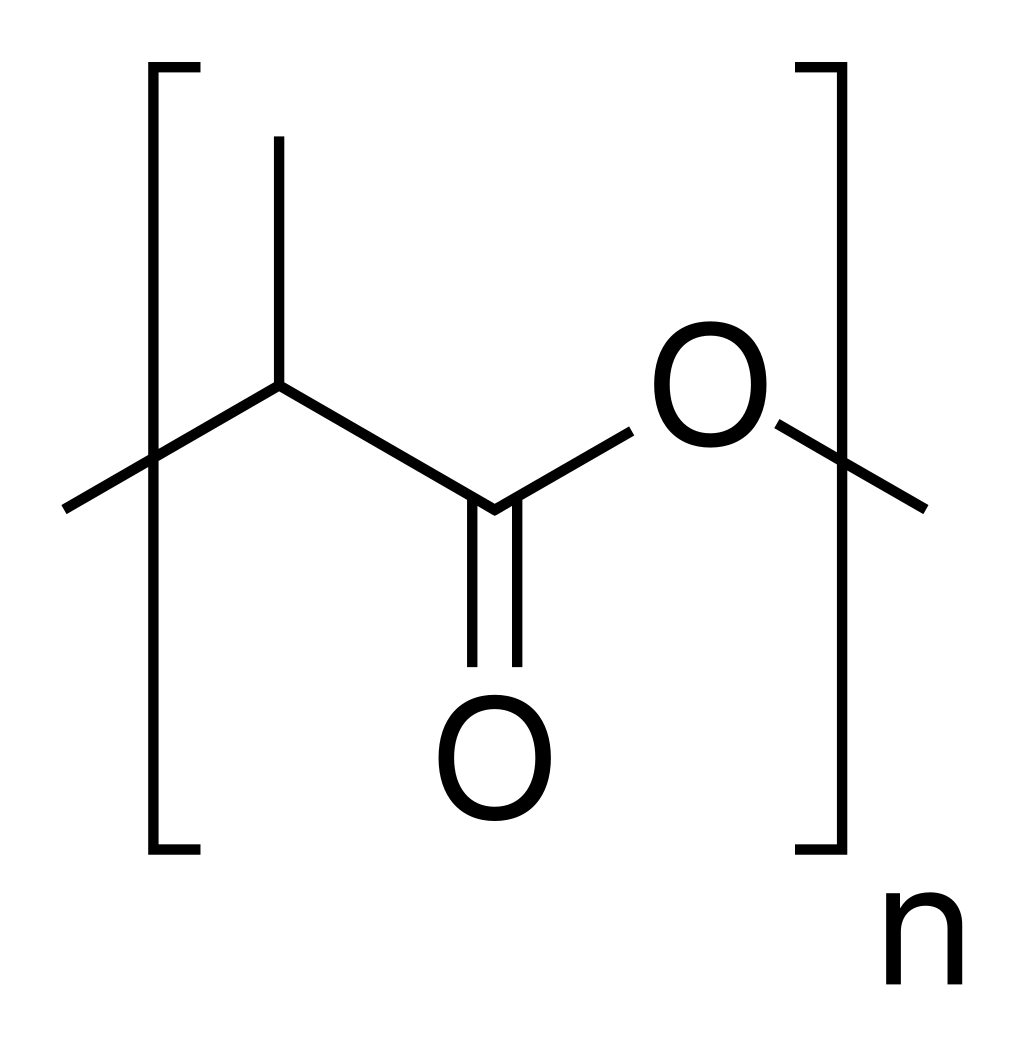
\includegraphics[width=0.65\linewidth]{img/pla_vzorec.png} 
	\end{subfigure}
	\begin{subfigure}{0.3\textwidth}
		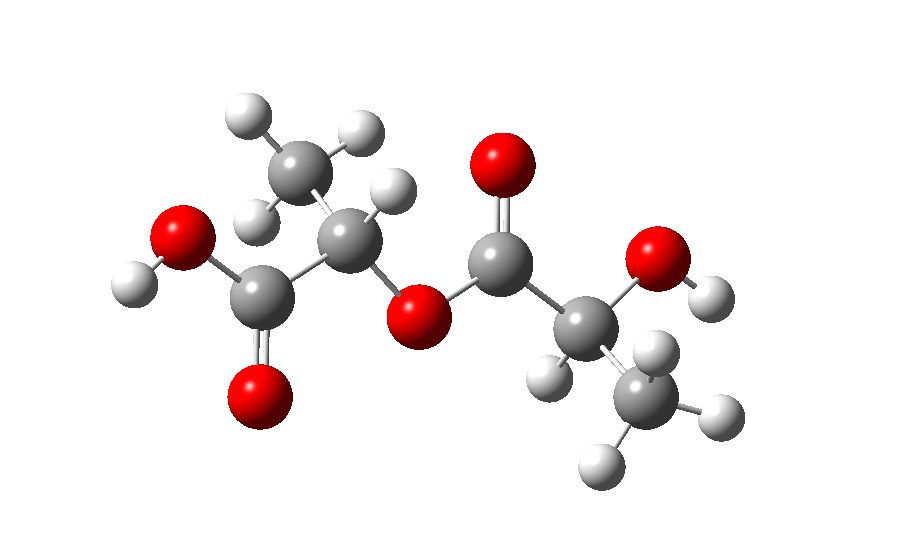
\includegraphics[width=1.2\linewidth]{img/pla_1d.png}
	\end{subfigure}
	\begin{subfigure}{0.33\textwidth}
		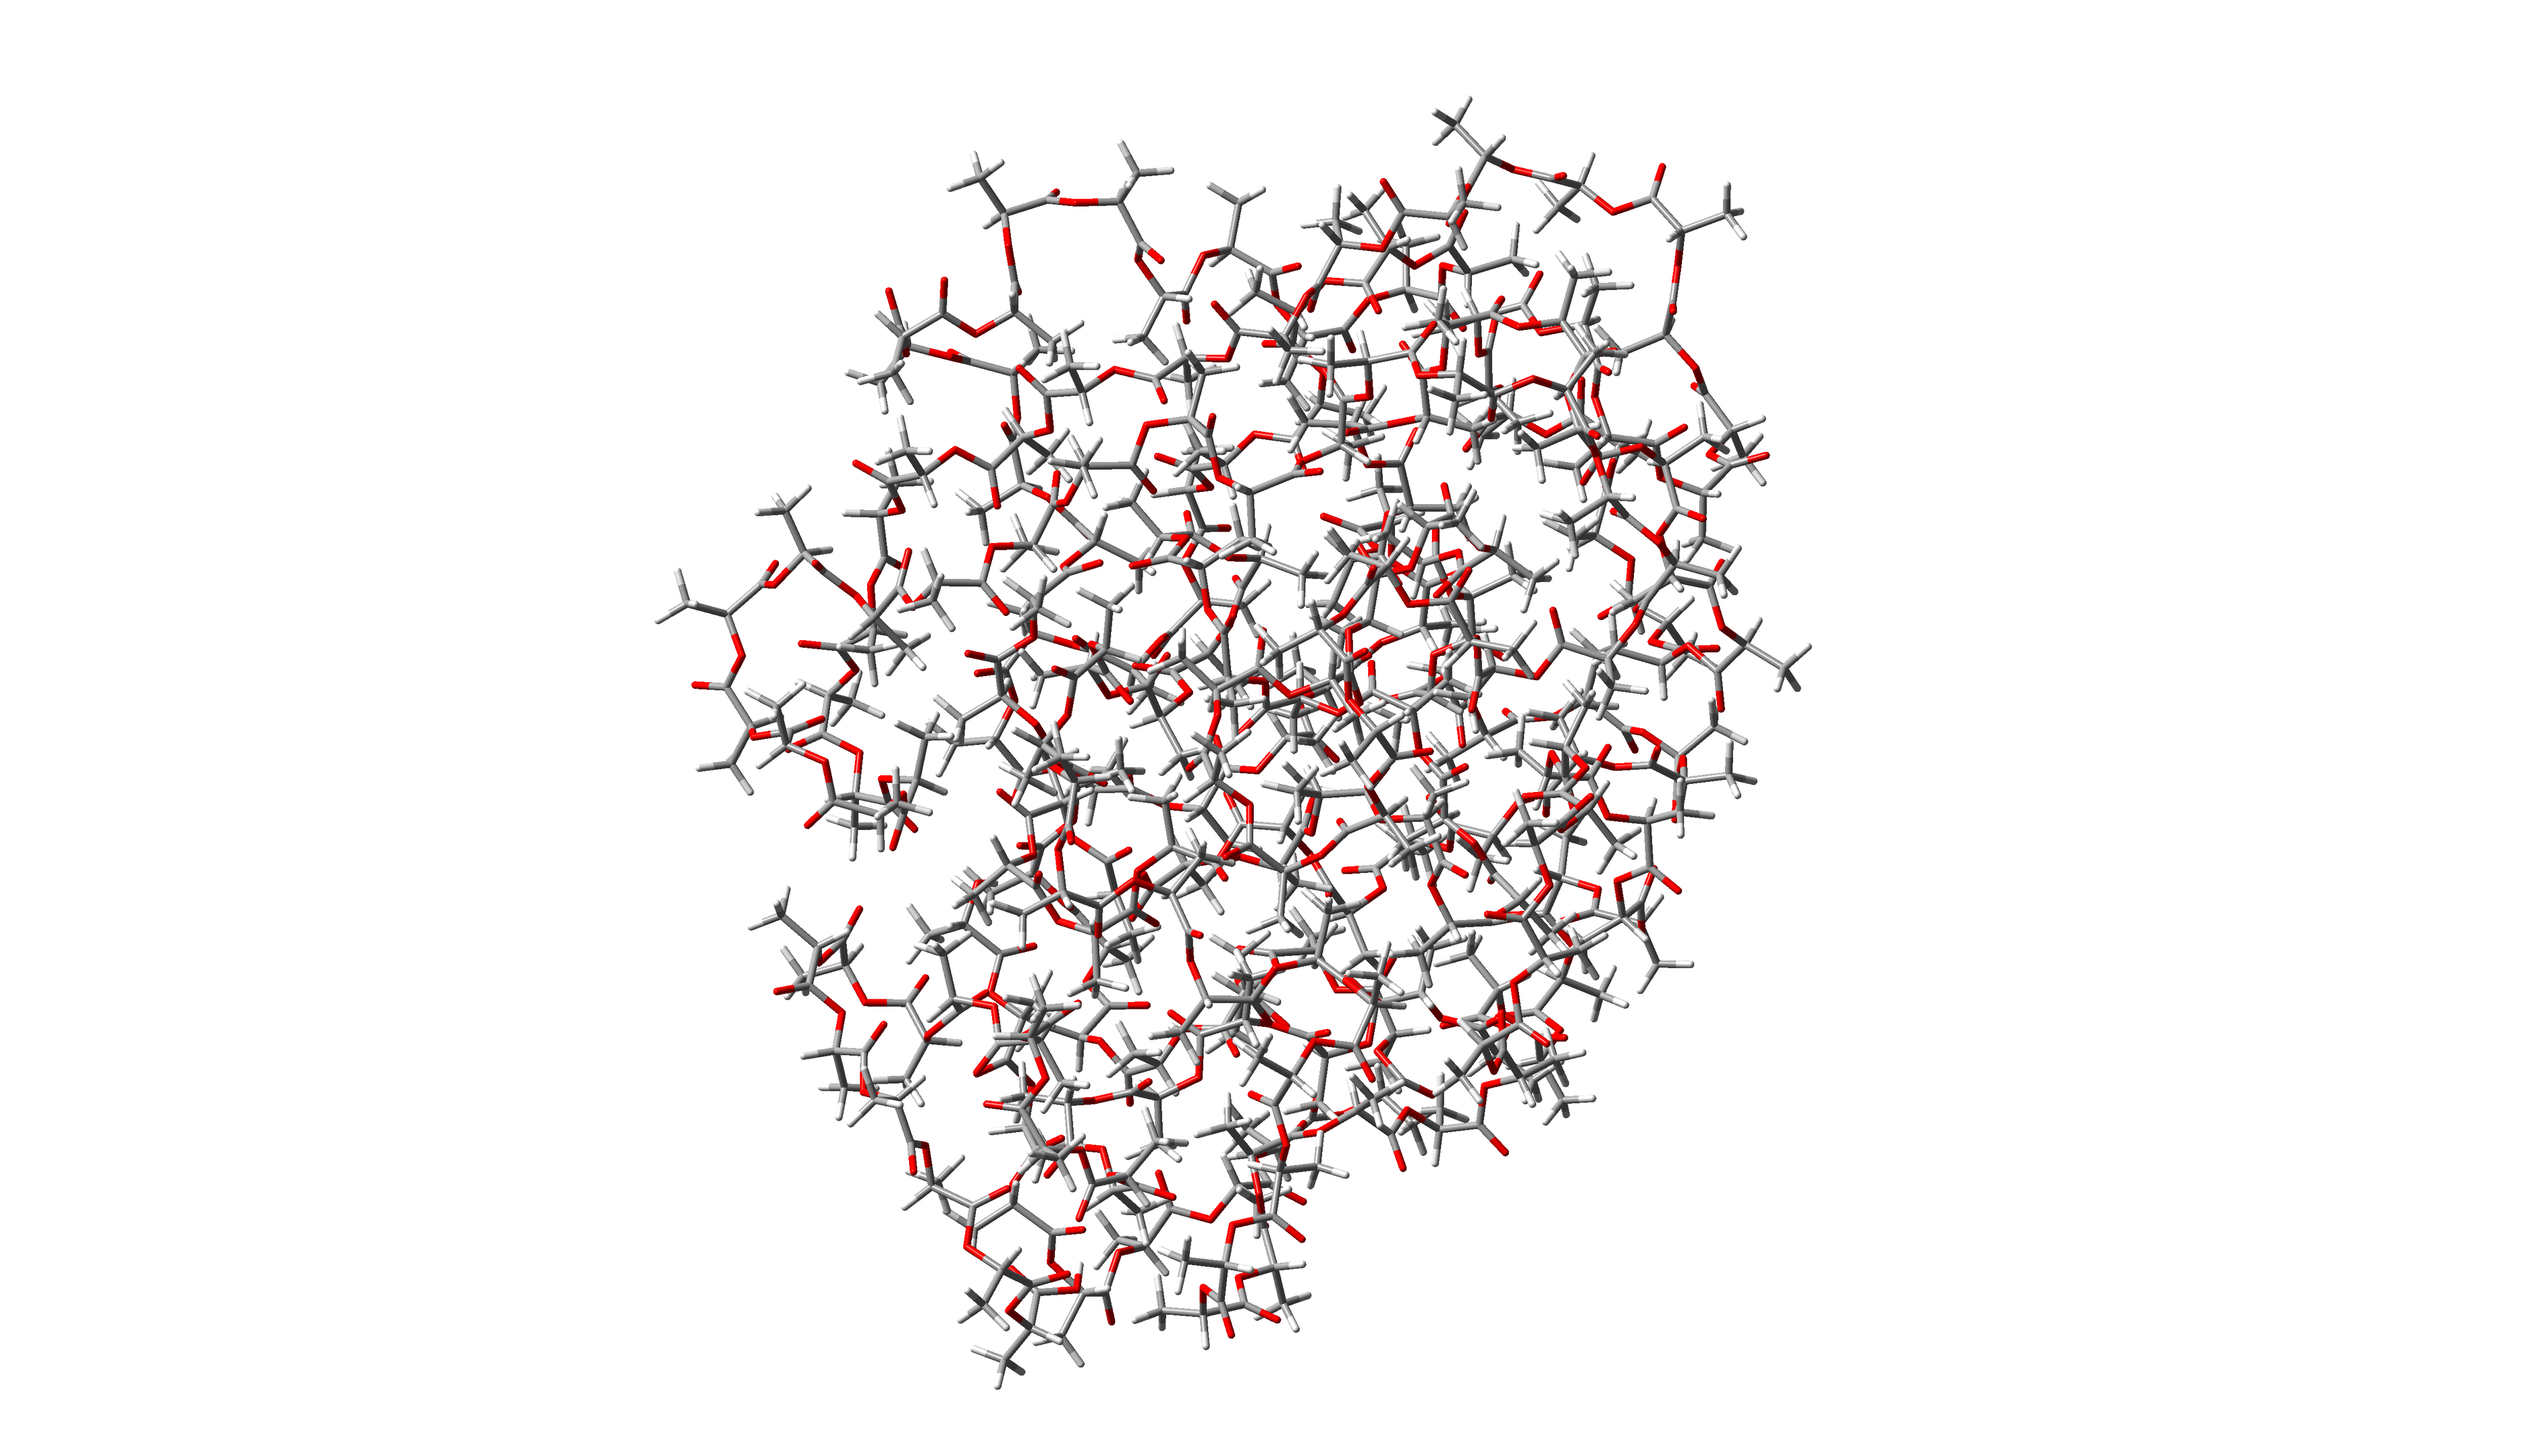
\includegraphics[width=1.4\linewidth]{img/pla_100g_tube.png}
	\end{subfigure}
	\caption{PLA formula on the left, PLA dimer block representing the chain unit used to build up polymer chain in the middle and a PLA chain containing 100 dimer block used to create mixtures with APIs on the right.}
	\vspace{-0.5cm}
	\label{fig:pla}
\end{figure}

\subsubsection{Active pharmaceutical ingredients}

%\subsubsection{Ibuprofen}
The first selected API is \textbf{ibuprofen}, systematically 2-(4-Isobutylphenyl)propanoic acid (C$_{13}$H$_{18}$O$_{2}$) as an example of a widely used analgesic-antipyretic-antiflammator drug. The racemic mixture is commonly used in medical treatment, whereas the S- enantiomer has stronger pharmaceutical activity than the R- enantiomer, which is metabolically transformed to S- in the organism. \cite{rainsford_ibuprofen_2009} In this work the S- form, which is visualised in Figure \ref{fig:APIs}, is used. The molar weight is $M_\mathrm{w}$~=~206.28~$\mathrm{g\ mol^{-1}}$ and the melting point is 324.4 K. \cite{stejfa_heat_2021} 

%\subsubsection{Naproxen}
The second selected API is \textbf{naproxen}, systematically 2-(6-Methoxynaphthalen-2-yl)propanoic acid (C$_{14}$H$_{14}$O$_{3}$), a non-steroidal anti-inflammatory drug, used as a painkiller. Naproxen contains three oxygen atoms (one carboxyl group and one ether bond), the structure is shown in Figure \ref{fig:APIs} in the upper right corner. On the basis of its structure, naproxen can donate one hydrogen bond and accept up to three hydrogen bonds. Naproxen is a white crystalline powder, with a molar weight of $M_\mathrm{w}$~=~230.263~$\mathrm{g\ mol^{-1}}$ and melting point 429.3 K. \cite{stejfa_heat_2021}

%\subsubsection{Carbamazepine}
\textbf{Carbamazepine}, alternatively 5-Carbamoyl-5H-dibenzo(b,f)azepine (C$_{15}$H$_{12}$N$_{2}$O) is a representative anticonvulsant, which is used for the treatment of seizures and neuropathic pain. Carbamazepine contains two nitrogen atoms (amide group) and one oxygen in the carboxyl group; its structure is shown in Figure \ref{fig:APIs} on the left side. According to its structure, carbamazepine can accept and donate one hydrogen bond. Carbamazepine is a white crystalline powder, with a molar weight of $M_\mathrm{w}$~=~236.273~$\mathrm{g\ mol^{-1}}$ and melting temperature of 463.6 K. \cite{stejfa_heat_2021}

%\subsubsection{Indomethacine}
\textbf{Indomethacin}, 2-{1-[(4-Chlorophenyl)carbonyl]-5-methoxy-2-methyl-1H-indol-3-yl}acetic acid (C$_{19}$H$_{16}$ClNO$_{4}$), which structure is in Figure \ref{fig:APIs}, is used in the treatment of musculoskeletal and joint disorders. The molar weight is $M_\mathrm{w}$~=~357.8~$\mathrm{g\ mol^{-1}}$ and the melting temperature is 433.3 K. \cite{stejfa_heat_2021}
\begin{figure}[htb!]
	%\centering
	\hspace{1.2cm}
	\subfloat{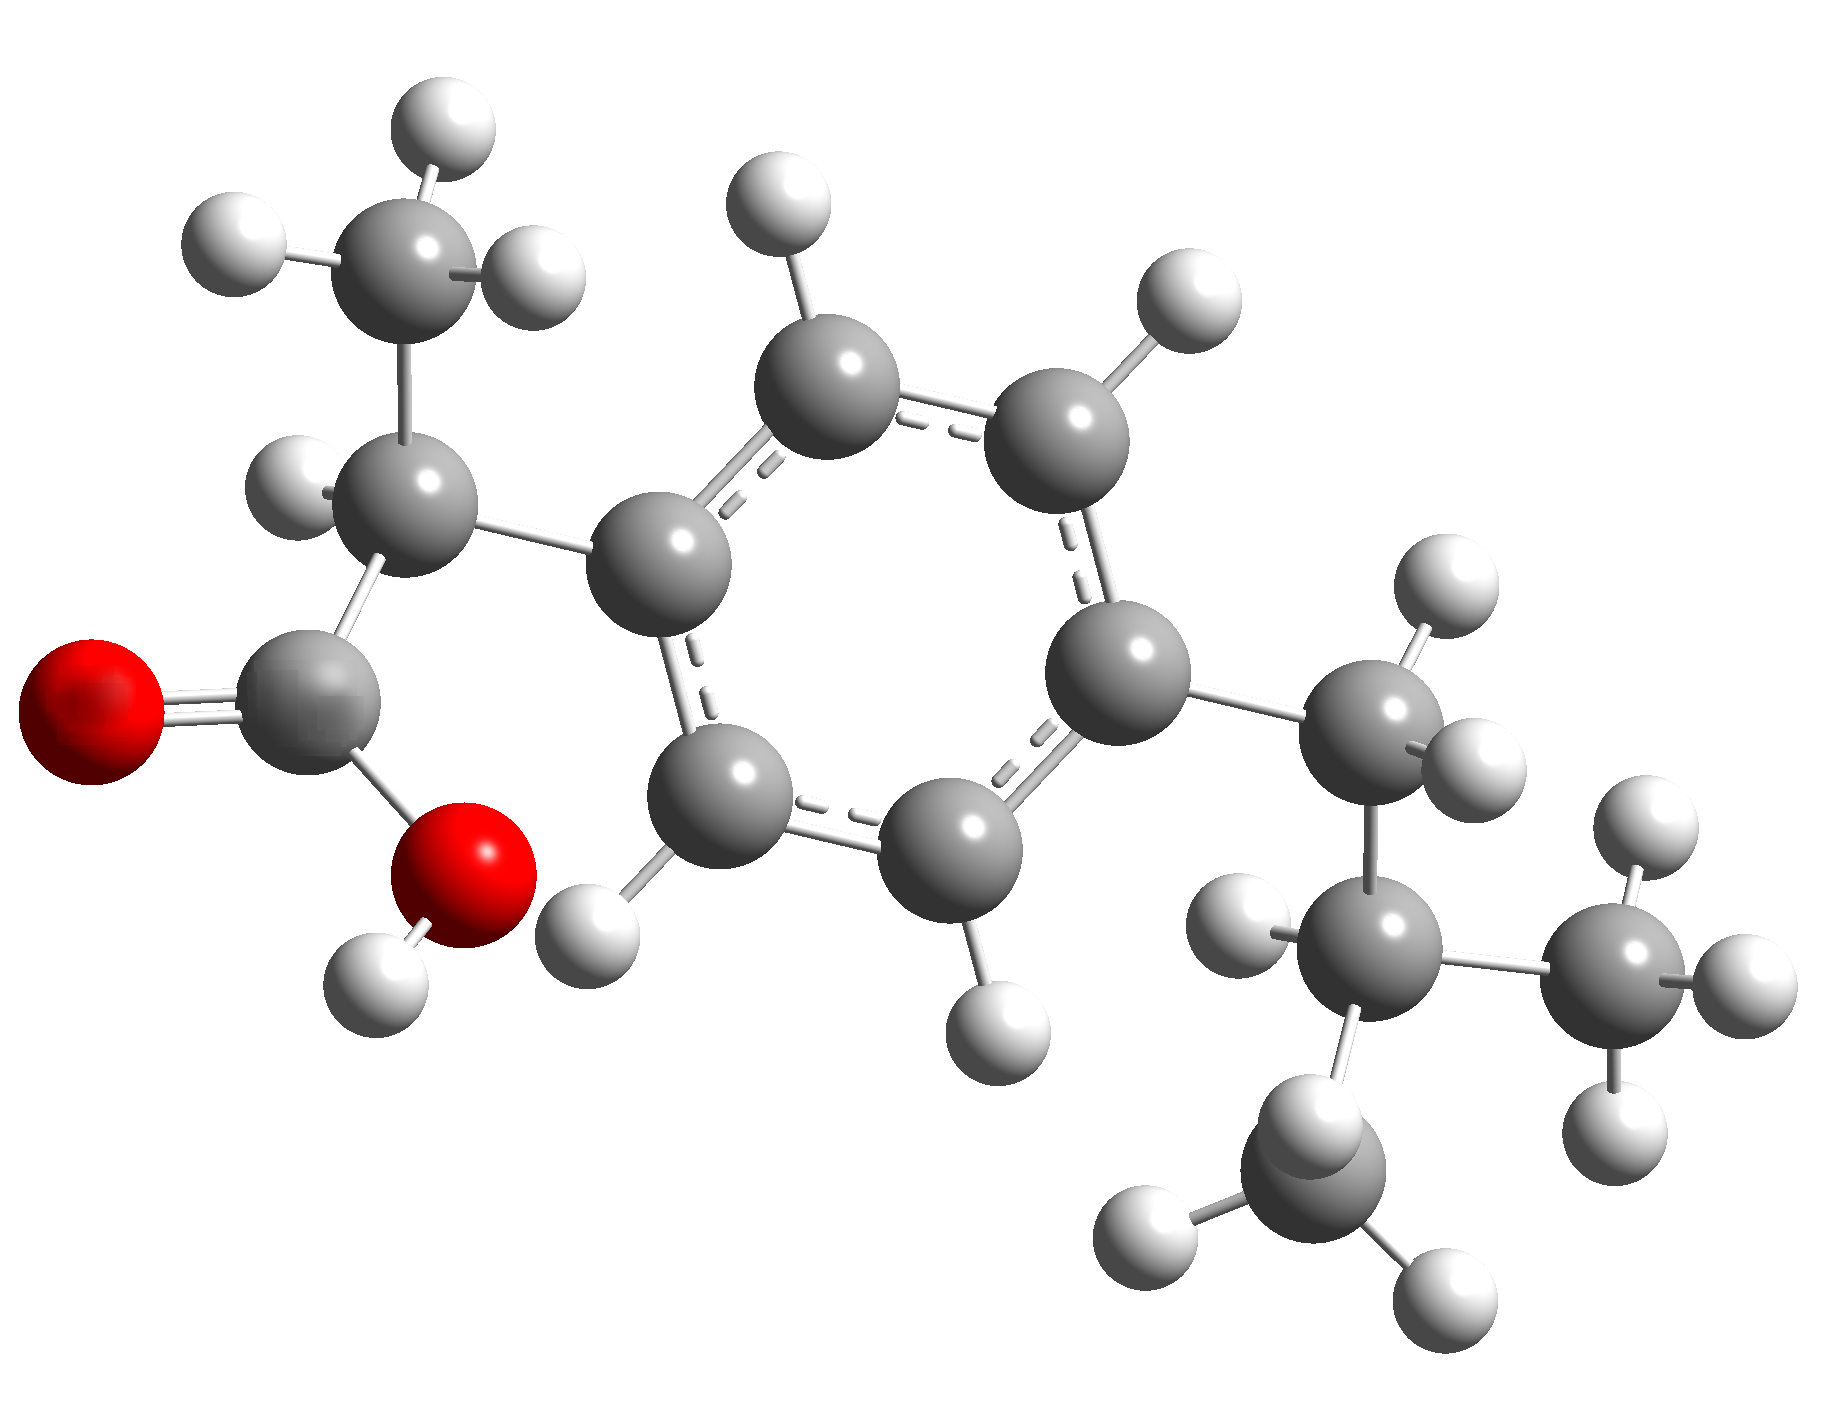
\includegraphics[width=0.35\linewidth]{img/ibu_s.png}}
	\hspace{2cm}
	\subfloat{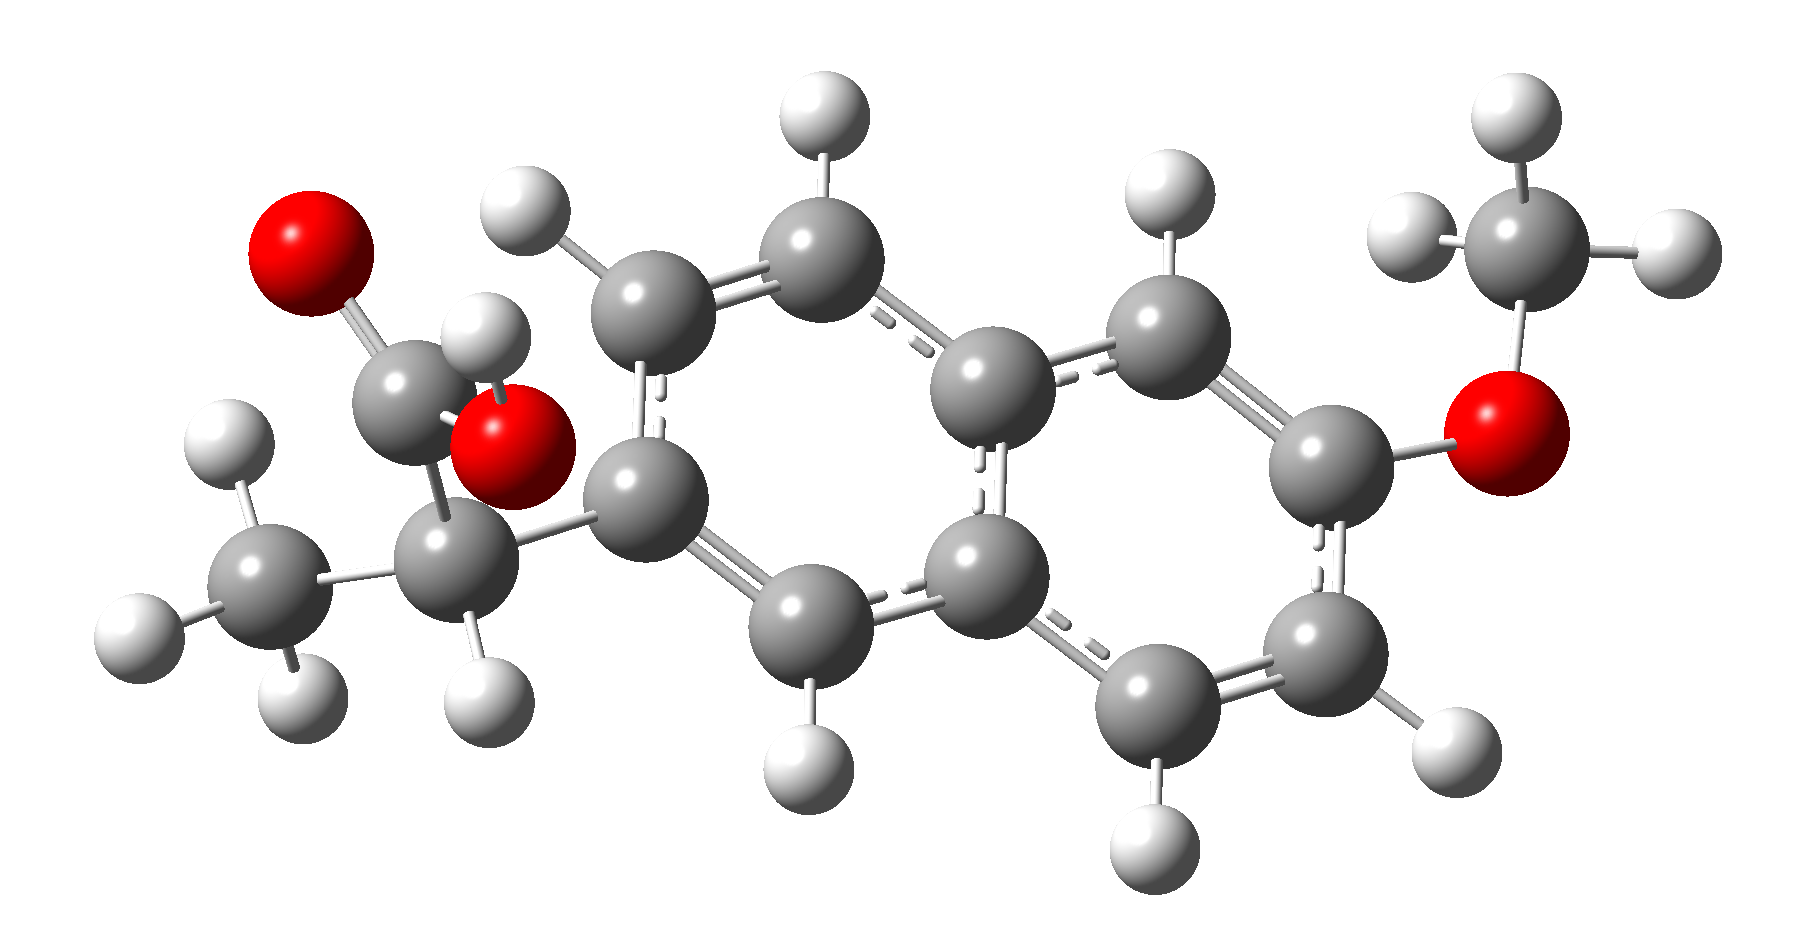
\includegraphics[width=0.45\linewidth]{img/nap.png}}\\
	\subfloat{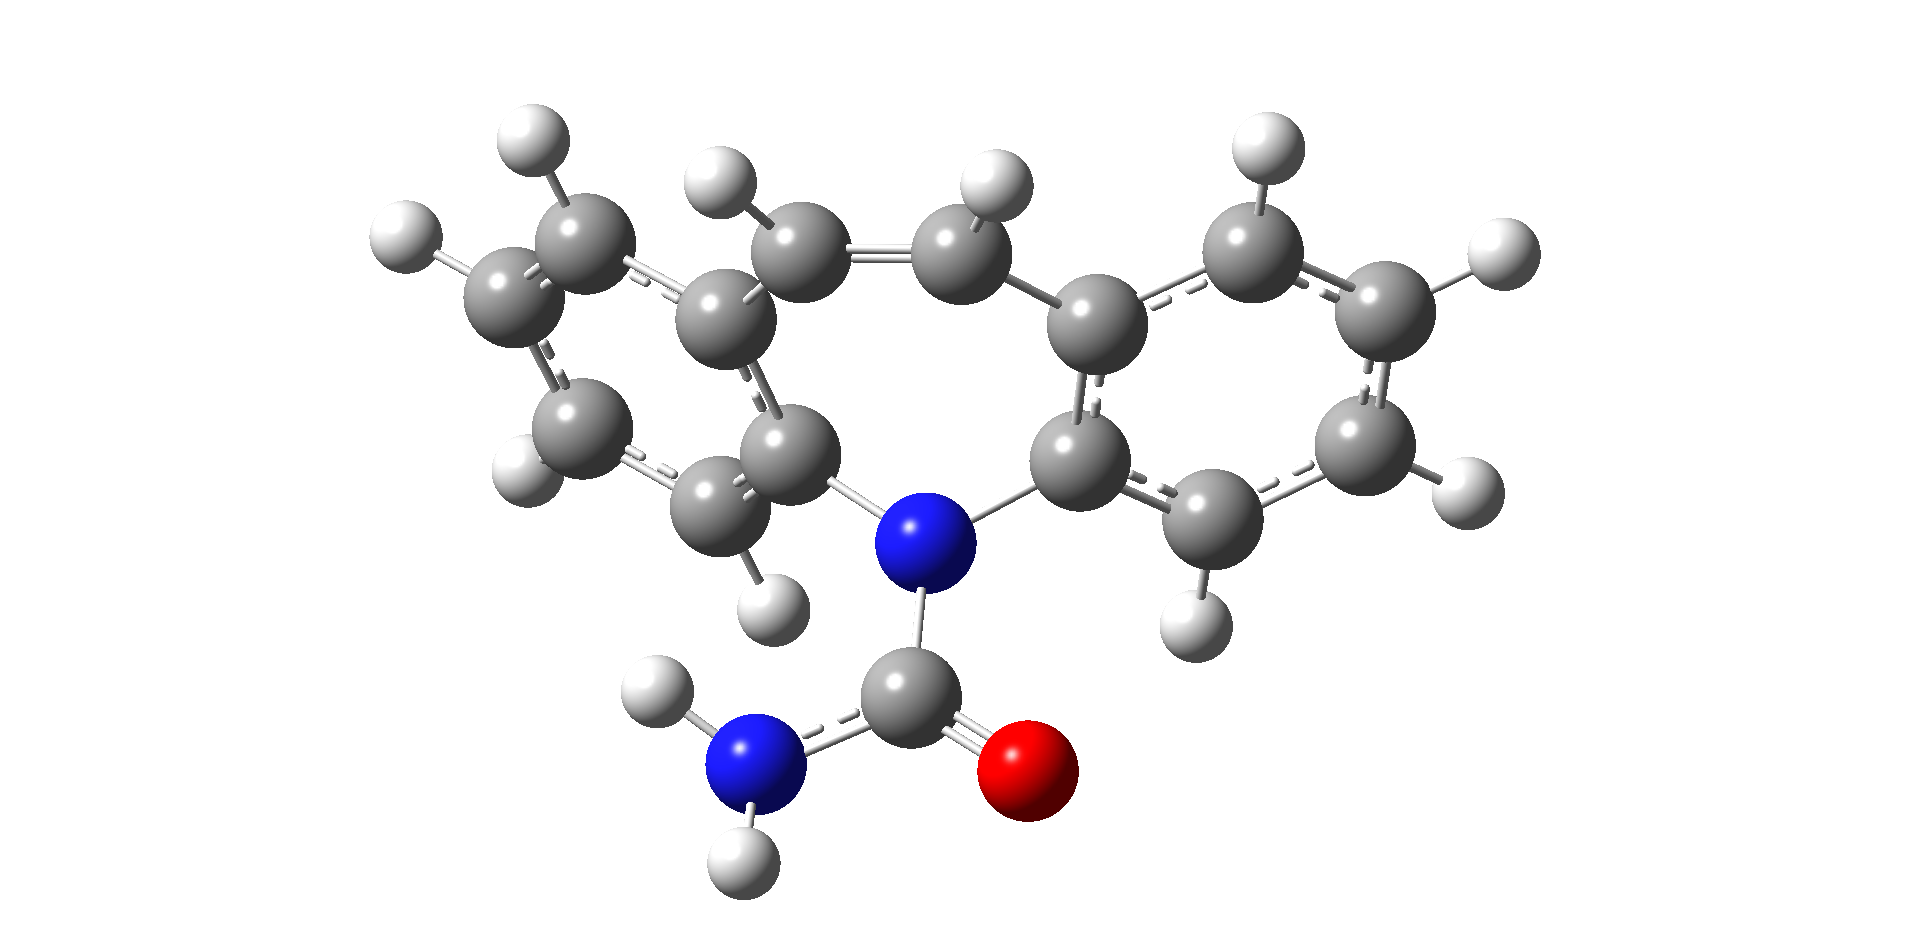
\includegraphics[width=0.6\linewidth]{img/cbz_svk.png}}
	\subfloat{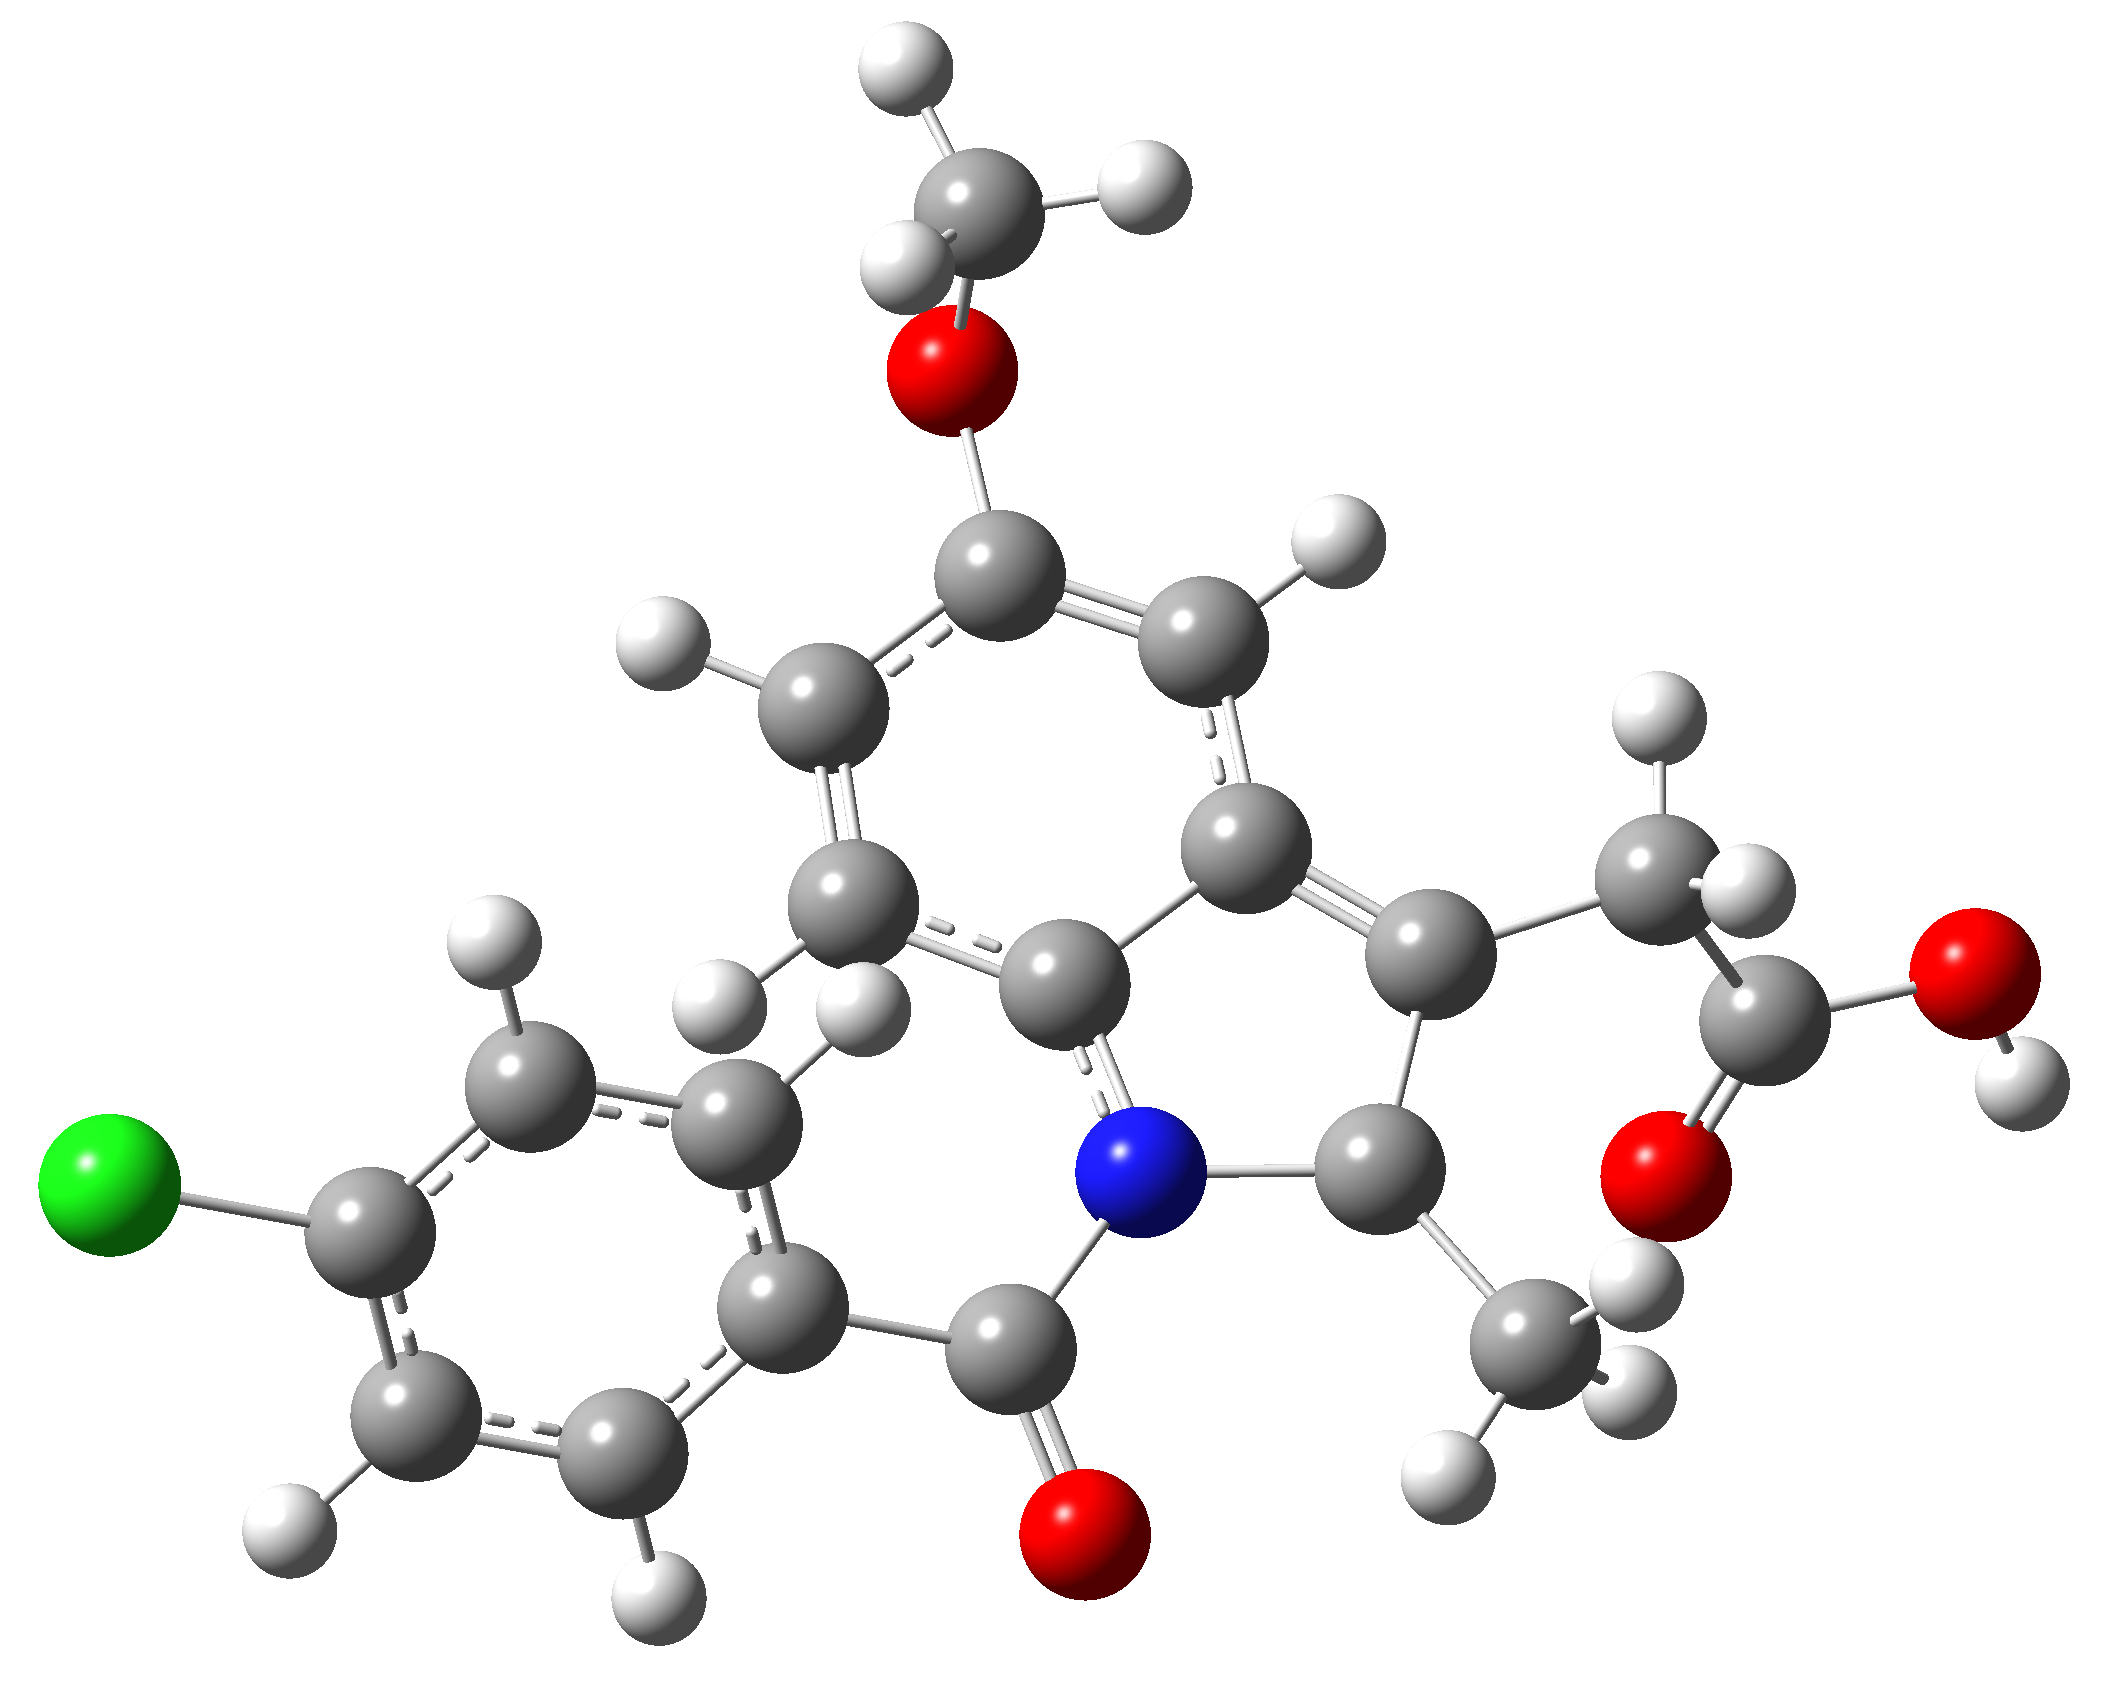
\includegraphics[width=0.4\linewidth]{img/indo.png}}
	\caption{Molecular structures of ibuprofen (\textbf{top left}), naproxen (\textbf{top right}), carbamazepine (\textbf{bottom left}) and indomethacin (\textbf{bottom right}).}
	\label{fig:APIs}
\end{figure}

%\subsubsection{Sulfathiazole}
The last selected API was \textbf{sulfathiazole} with systematic name 4-amino-N-thiazol-2-ylidenebenzene-sulfonamide as a representative antibiotic drug from the sulfonamides group, which is used in the treatment of pyogenic cutaneous infections. Sulfathiazole is a white crystalline powder, with a molar weight $(M_\mathrm{w})$ =255.3 $\mathrm{gmol^{-1}}$, which is highly polymorphic, five polymorphs have been discovered so far \cite{caron_comparison_2011}. All known polymorphs of sulfathiazole crystallise in the $P2_1/c$ space group, but there are differences in intermolecular bonding and structural properties \cite{drebushchak_crystal_2008}. The II polymorph structure, shown in Figure \ref{fig:sulfathiazole}, is used in this work. There are four molecules of sulfathiazole in the crystal monoclinic unit cell. 

\begin{figure}[htb!]
	\begin{subfigure}{0.5\textwidth}
		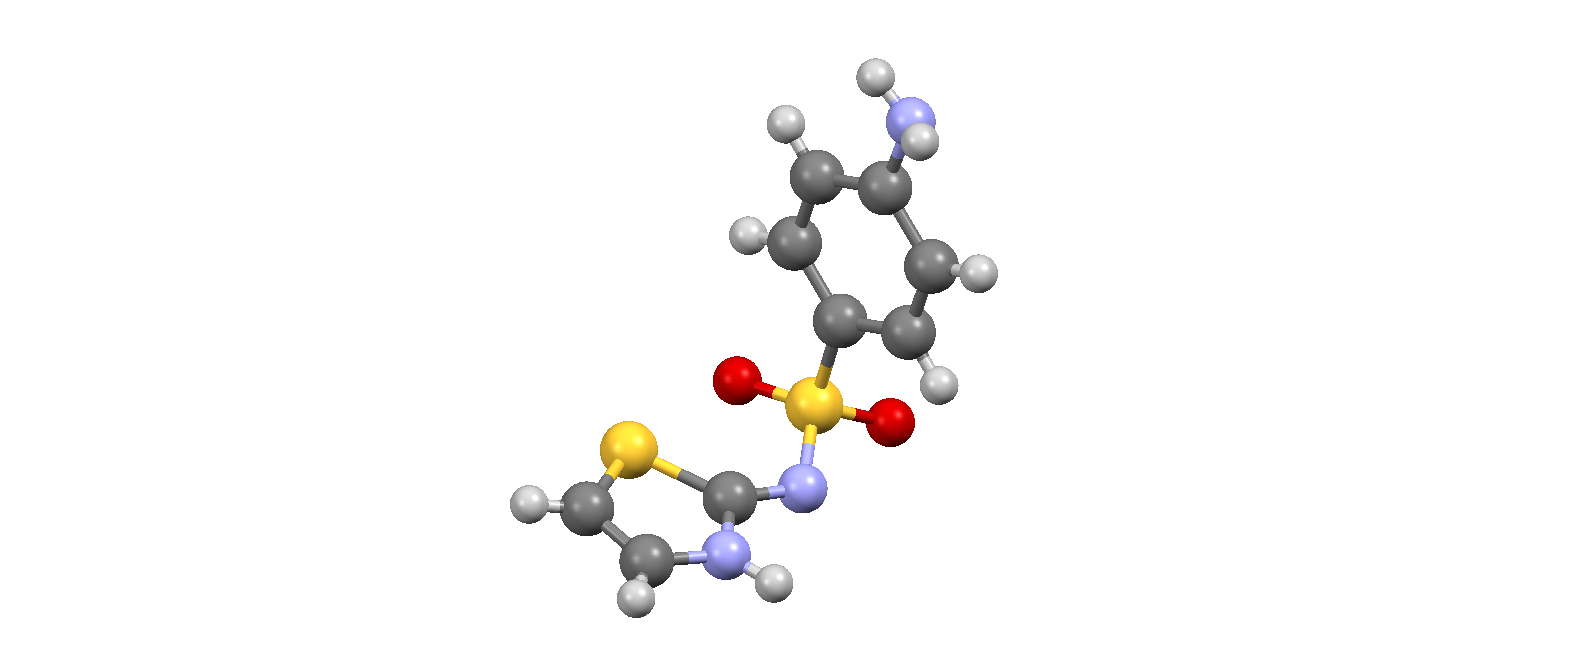
\includegraphics[width=1.2\linewidth]{img/sulfathiazol.png} 
	\end{subfigure}
	\begin{subfigure}{0.5\textwidth}
		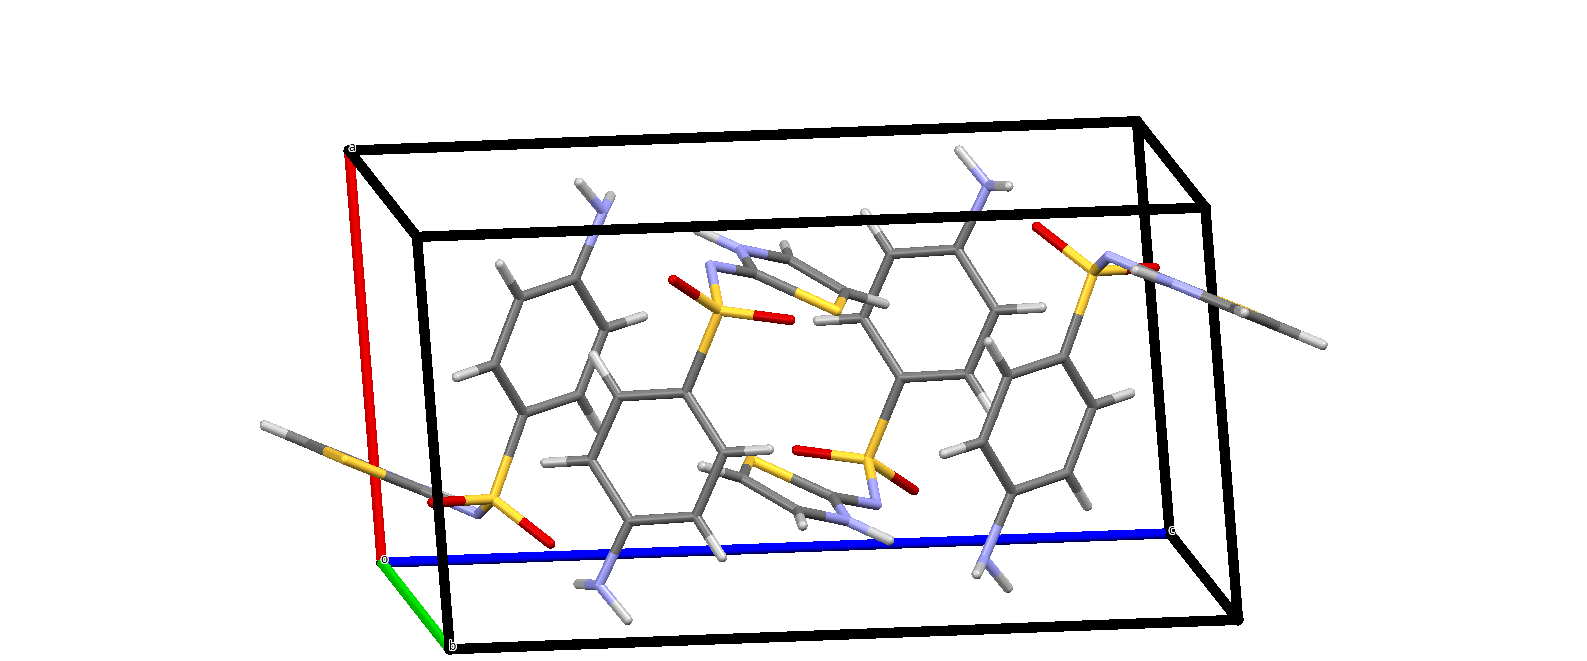
\includegraphics[width=1.1\linewidth]{img/sulfathiazol_packing.png}
	\end{subfigure}
	\caption{Sulfathiazole - molecular structure on the left and a unit cell of its II polymorph on the right.}
	\label{fig:sulfathiazole}
\end{figure}

\subsection{Objective}



% %%%%%%%%%%%%%%%%%%%%%%%%%%%%%%%%%%%%%%%%%%%%%%%%%%%%%%%%%%%%%%%%%%%%%%%%%
\newpage
\section{THEORETICAL PART}

%%%%%%%%%%%%%%%%%%%%%%%%%%%%%%%%%%%%%%%%%%%%%%%%%%%%%%%%%%%%%%%%%%%%%%%%%%%%%%%%%%%%%%%%
%%%%%%%%%%%%%%%%%%%%%%%%%%%%%%%%%%%%%%%%%%%%%%%%%%%%%%%%%%%%%%%%%%%%%%%%%%%%%%%%%%%%%%%%
In order to convert a real system consisting of individual molecules into a form that can be understood by a computer software, we must define individual parameters that are essential for describing mutual interactions of atoms. When describing real systems, it is usually necessary to consider a certain degree of approximation due to the possible computational complexity. In computational chemistry methods, we often encounter the so-called Born-Oppenheimer approximation, which is based on the decoupling of the motion of nuclei and electrons. The basis of the approximation is the orders-of-magnitude difference in mass between the electron and the nucleus. The latter thus move very slowly relative to the electrons and can thus be considered as a fixed point charge. This allows us to calculate the energy of a molecule as a function of the positions of the nuclei, in quantum chemistry we talk about the so-called Potential Energy Surface (PES), which is a function of 3$N$ coordinates, where $N$ is the number of nuclei. \cite{leach_molecular_2001} 

For small systems it is possible to calculate the PES based on quantum chemistry methods using reasonable resources, for very large systems this is not yet realistic. We therefore introduce a classical-mechanics set of analytic functions, yet empiric parameters called the Force Field (FF), which enable to evaluate the energy of simulated systems depending on the positions of the nuclei. Methods based on the use of such Force Fields are called molecular mechanics, which are applied especially when quantum phenomena are not of great importance and we can use classical mechanics approach or big amorphous systems where quantum-based calculations would be extremely expensive and resource taking. \cite{monticelli_force_2013}

\subsection{Force fields}
The total energy calculated using the force field can be broken down into two contributions, a binding and a non-binding term, which are further expanded in Equations \ref{eq:ff2} and \ref{eq:ff3}.

\begin{comment}
	\begin{equation}\label{eq:ff1}
		E_{\text{total}} = E_{\text{bonded}} + E_{\text{nonbonded}}
	\end{equation}.
\end{comment}


\begin{equation}\label{eq:ff2}
	E_{\text{bonded}} = E_{\text{bond}} + E_{\text{angle}} + E_{\text{torsion}}
\end{equation}

\begin{equation}\label{eq:ff3}
	E_{\text{nonbonded}} = E_{\text{electrostatic}} + E_{\text{Van der Walls}}
\end{equation}

%To get a better idea of what lies behind the individual terms, visualization of the corresponding mechanistic degrees of freedom is in the Figure \ref{fig:ff}. OBRÁZEK VYTVOŘÍM VLASTNÍ V PODOBNÉM DUCHU----
%
%\begin{figure}[htb!]
%	\centering
%	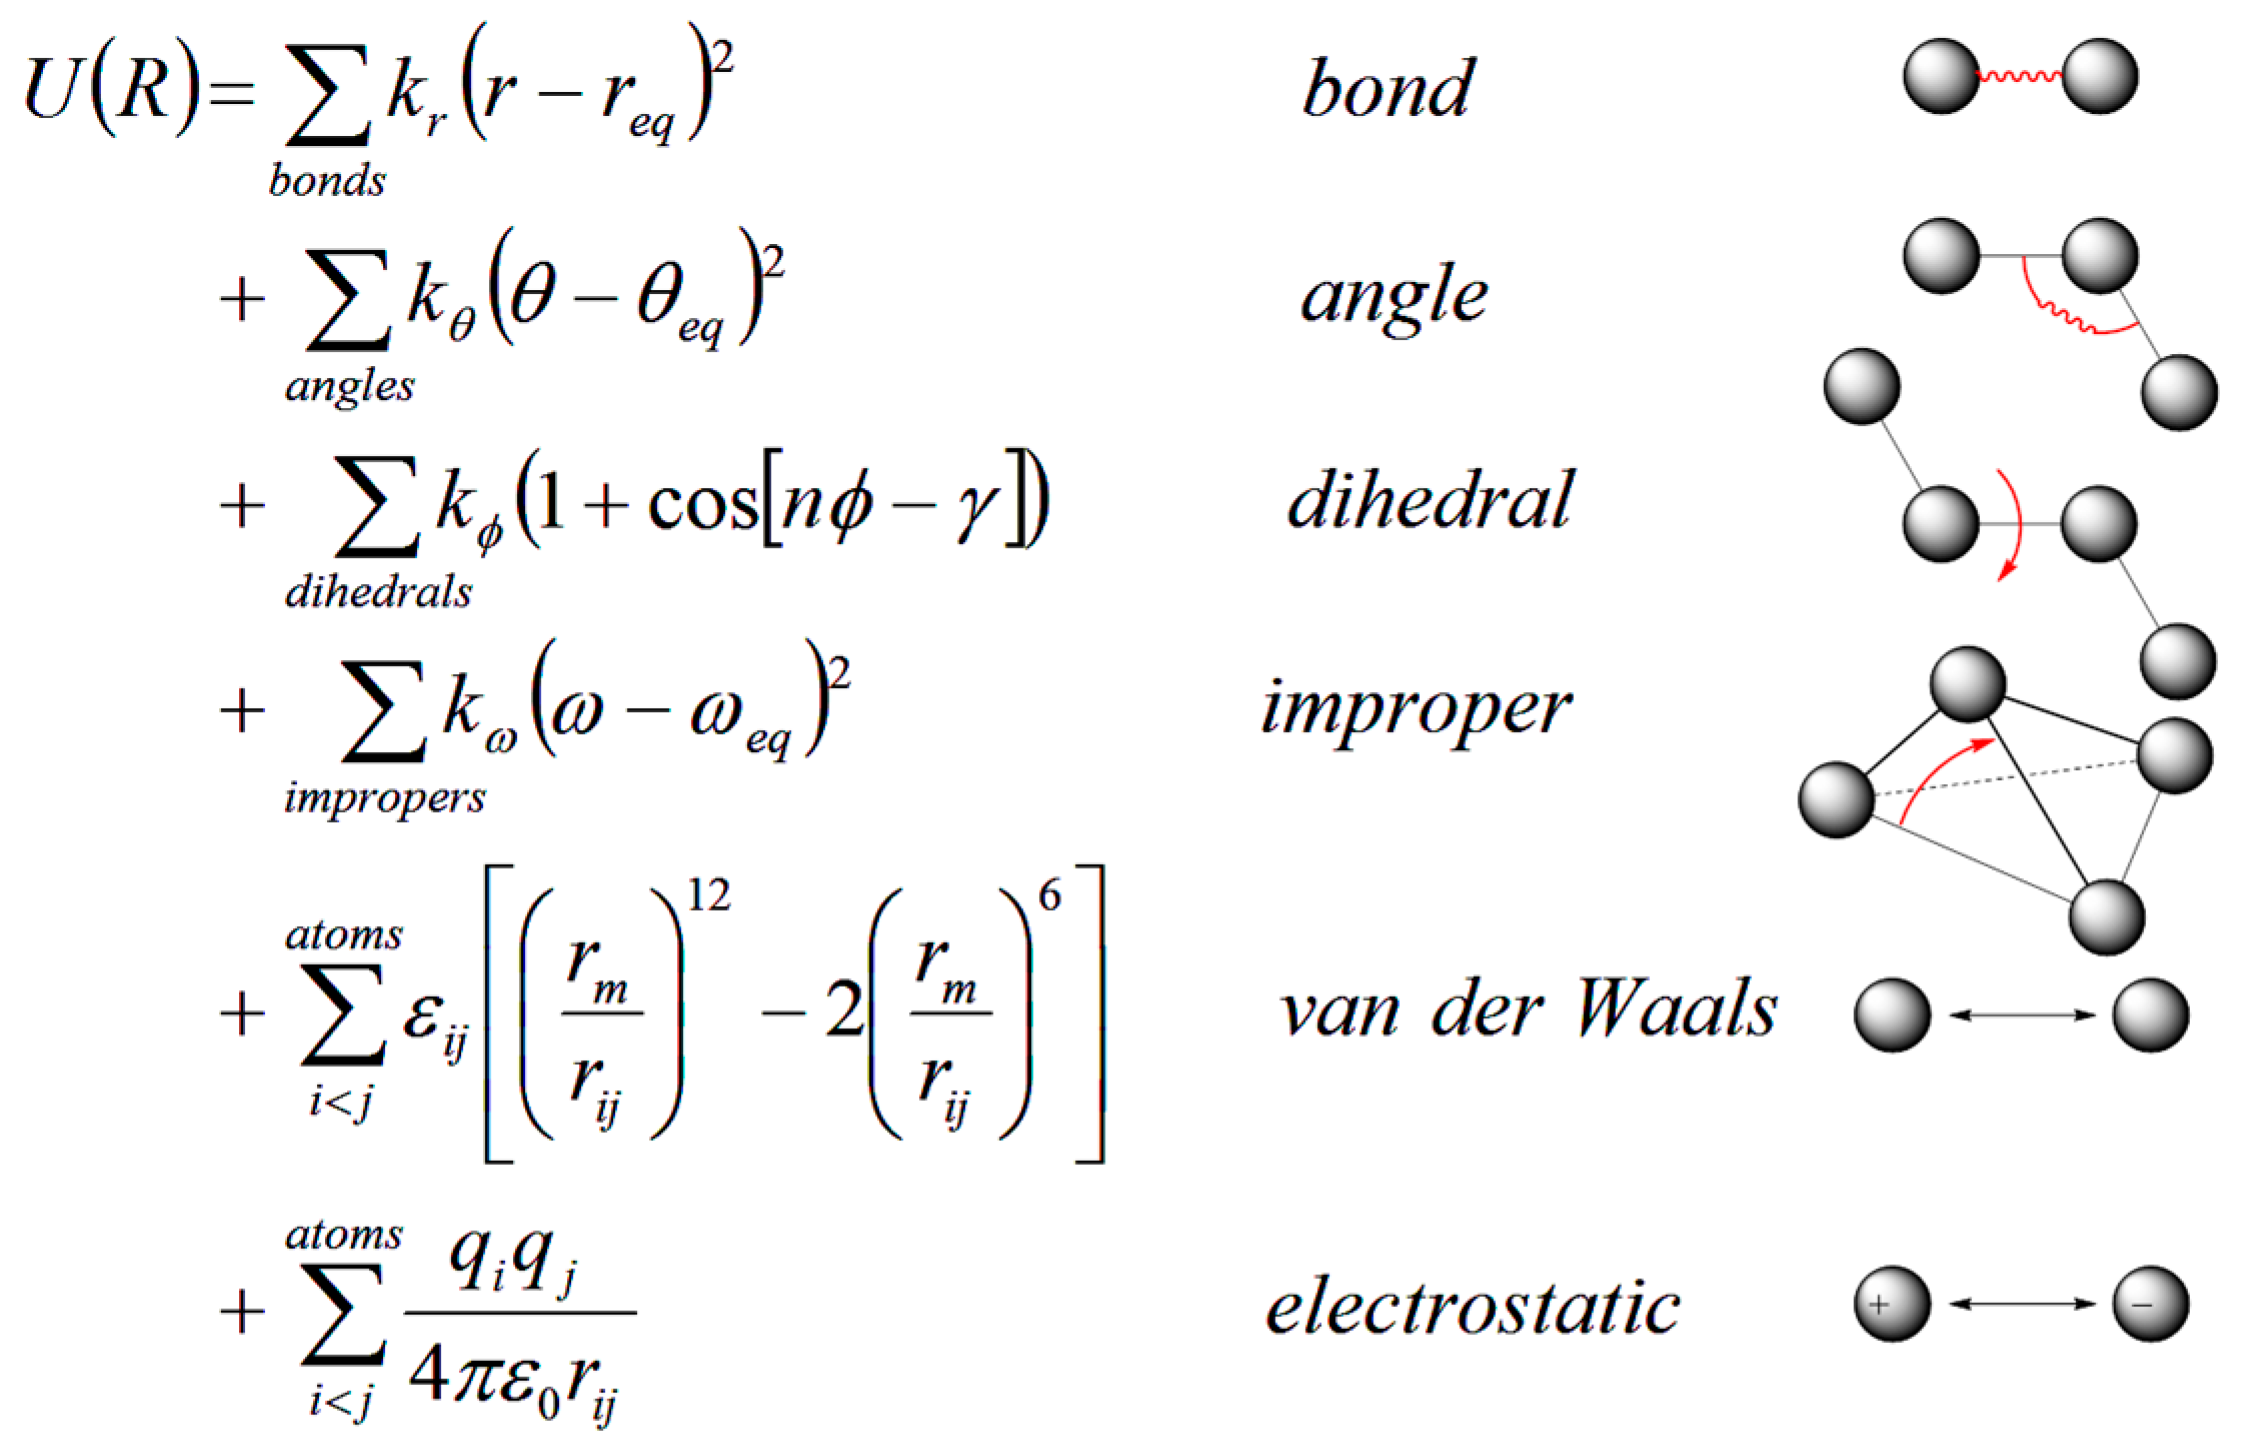
\includegraphics[width=1.0\linewidth]{img/ff.png} 
%	\caption{caption}
%	\label{fig:ff}    
%\end{figure}  

By the level of functional description (number of terms) of the interactions in the force field, we distinguish force fields of three classes. Class 1 force fields contain the 5 terms mentioned in the two equations above (bond, angle, torsion, Lennard-Jones and electrostatic), examples of such FF are the DREIDING, AMBER \cite{brooks_charmm_2009}, GAFF and OPLS. In addition, class 2 force fields include bond-bond and bond-angle coupling terms, anharmonic terms simultaneously with all class 1 terms, examples of such fields are PCFF or ReaxFF.  The third class includes fluctuations of charge distribution in time (charge polarization effect), and they are called polarizable FF. \cite{vanommeslaeghe_molecular_2014}

During the parameterization of force fields (FF), we start from the assumption of transferability,  similar chemical groups of different molecules interact in the same way. When constructing a force field for large molecules, we can use parameters obtained from data for small molecules, which are much more easily graspable and contain the same functional groups. \cite{monticelli_force_2013} In model development, our aim is to achieve the most universal description of the system while still closely corresponding to its actual state. This can be facilitated by employing higher-order terms; however, incorporating anharmonic and cross terms introduces the need for a greater amount of FF parameters. We strive to avoid situations where we employ an overly adapted and detailed model that merely reproduces inserted information without providing any predictive capabilities. \cite{vanommeslaeghe_molecular_2014}

According to the level of parameterization, there are 3 basic types of force fields. In the first case, where the parameters are determined for each individual atom in the system, including hydrogens, we speak of an all-atom force field. A united atom force field is one where we parameterize the individual functional groups (interaction centers), such an interaction center could be for example a methyl group. The third type of force field is coarse grained, used mainly for protein and polymer simulations, offering higher computational efficiency for long simulations of large molecules by grouping them into "superatoms". \cite{da_silva_are_2020}

\subsubsection{OPLS force field}

Optimized Potential for Liquid Simulations (OPLS) force field was developed by William L. Jorgensen \cite{jorgensen_opls_1988} at Purdue University and later at Yale University based on previously released Assisted Model Building and Energy Refinement (AMBER) force field developed by Peter Kollman's group. \cite{cornell_second_1995} The OPLS force field consists of following terms written in Equation \ref{eq:opls}. 
	
	\begin{equation}
		\begin{aligned}
			U_{\text{OPLS}} = & \sum_{\text{bonds}} \frac{1}{2} k_b(r-r_0)^2 + \sum_{\text{angles}} k_{\theta} (\theta-\theta_0)^2 \\
			& + \sum_{\text{torsions}} \Biggl( \frac {V_1} {2} \left [ 1 + \cos (\phi) \right ] + \frac {V_2} {2} \left [ 1 - \cos (2\phi) \right ] 
			+ \frac {V_3} {2} \left [ 1 + \cos (3\phi) \right ] + \frac {V_4} {2} \left [ 1 - \cos (4\phi) \right ] \Biggr) \\
			& + \sum_{i=1}^{N-1} \sum_{j=i+1}^N \left\lbrace 4\epsilon_{ij} \left[ \left( \frac{\sigma_{ij}}{r_{ij}} \right)^{12} - \left( \frac{\sigma_{ij}}{r_{ij}} \right)^6 \right] + \frac{q_iq_je^2}{r_{ij}} \right\rbrace f_{ij}
		\end{aligned}
		\label{eq:opls}
	\end{equation}
	
$i$ and $j$ denote different atom types, $N$ is the total number of atom pairs, $\epsilon_{ij}$, $\sigma_{ij}$ are LJ parameters, $r_{ij}$ is the distance between atoms $i$ and $j$, and $f_{ij}$ is scaling factor equals 0.5 for 1-4 interactions ($i,j$=1,4) and 1 otherwise.
	
\textbf{Bonds and angles} are described as harmonic oscillators in OPLS FF. The equilibrium parameters are obtained by structural methods, such as x-ray diffraction NMR experiments. The values for force constants are then fitted to experimental data taken from vibrational spectroscopy. In Figure \ref{fig:bond} is the visualization of the constants.

\begin{figure}[htb!]
	\centering
	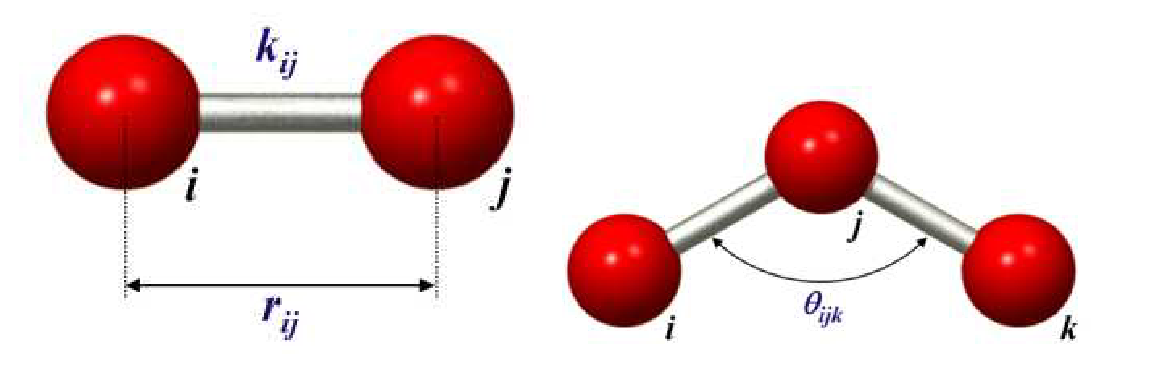
\includegraphics[width=1.0\linewidth]{img/bond_angles.png} 
	\caption{caption}
	\label{fig:bond}    
\end{figure}   

Proper \textbf{dihedral angle} $\phi$ between atoms i,j,k,l is represented in Figure \ref{fig:torsion}. The torsional energy is described as a cosine expansion, where the first term corresponds to the rotation periodic after 360$^\circ$, second term by 180$^\circ$, the third term by 120$^\circ$ and the fourth term by 90$^\circ$. Each of this term has the $V_n$ constant, representing the barrier for rotation along the proper dihedral angle, which is dependent both on the torsional energy and non-bonded forces. Different approaches could be chosen, one of them is obtaining the parameters by QM calculations. \cite{mackerell_empirical_2004} We first optimize the molecular geometry using QM methods and then we run scanning of dihedral angle of interest. At each step, we optimize geometry and calculate the change in potential energy.  Then we compute potential energy of each optimized geometry using MD with dihedral parameters set to zero. Then we can fit the parameters by subtracting the results of MD from QM, this corresponds exactly to the influence of dihedrals. To do this procedure first all the other FF parameters should be known. 

\begin{figure}[htb!]
	\centering
	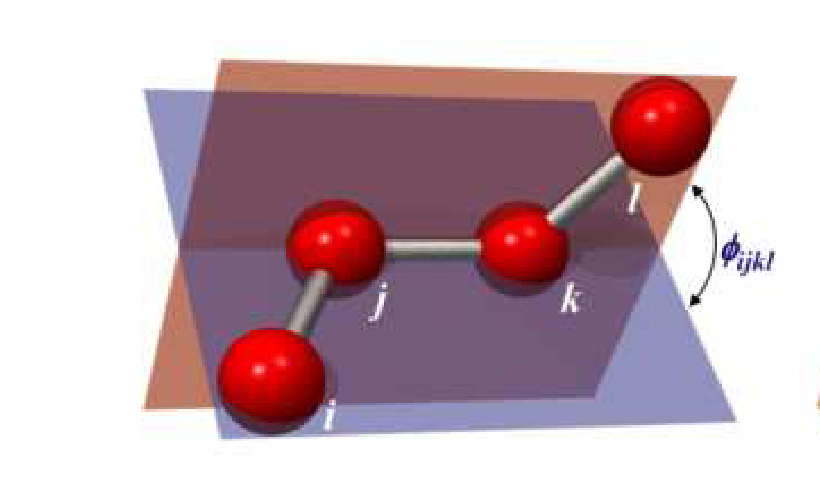
\includegraphics[width=1.0\linewidth]{img/torsion.png} 
	\caption{caption}
	\label{fig:torsion}    
\end{figure}   

\textbf{Charges} parametrization is also done by ab initio methods. When we are using the classical FF, the charges used to calculate the Coulomb potential remains the same during the simulations. Due to that, it is crucial to obtain the charges from equilibrium state of the molecules in order to avoid any errors from having the charges taken from structures with higher energy. When obtaining the charges, the first step is to optimize the geometry using the appropriate level of theory, meaning the basis set to be better or equal to 6-31G. Commonly used method to achieve the charges is CHELPG (CHarges from ELectrostatic Potentials using a Grid based method) \cite{breneman_determining_1990}, based on adjusting the partial charges at the centers of the nuclei in order to get the best representation of the electrostatic potential given by the wave functions. Calculation of the charges are often done using higher-level methods and basis sets such as B3LYP/cc-pVTZ or HF/6-31G**.

\textbf{Van der Waals} forces are most often represented by the Lennard-Jones (LJ) potential. The functional form with the illustration is in Figure \ref{fig:lj}. Lennard-Jones potential is a combination of two terms, repulsive term describes the Pauli repulsion at short distances and the attractive term describes the London dispersion force. The $\epsilon$ values are adjusted to experimental values of heats of vaporization and $\sigma$ parameters are adjusted to experimental densities and structural data. 

\begin{figure}[htb!]
	\centering
	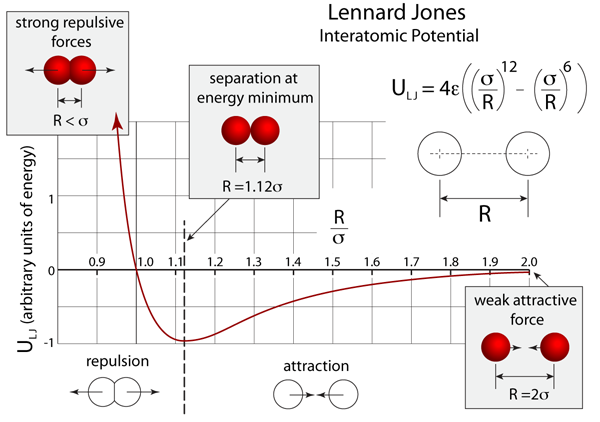
\includegraphics[width=1.0\linewidth]{img/lj.png} 
	\caption{caption}
	\label{fig:lj}    
\end{figure} 


\subsubsection{Polarizability}



\subsection{Periodic boundary conditions}
Due to the computational complexity, we are focused on only small region of a very complex real system.  In order not to introduce errors caused by the boundaries of the system and interaction on them, we introduce periodic boundary conditions (PBC). This method is based on surrounding the simulated system with periodic images, thus achieving an approximation by a surface less system. We choose a shape of the simulation box that can be used to fill the space without problems, in our case a cubic box. For simulations in three dimensions, we usually introduce PBCs in the direction of all axes, which means that our simulated box is surrounded on all sides by a total of 26 replicas of the system. The behavior of the system is the same in all replicas, so we must include all the particles appearing in the replicas when calculating the pair interactions. 

\subsubsection{Setting the cutoff}
From the preceding paragraphs it is evident that the main problem in time complexity of the simulations is the evaluation of non-bonding energies. While the number of bonded terms increase linearly with the system size, the non-bonded terms show a quadratic increase in the number of contributions. A common strategy for reducing the computational time is to set specific cutoff distance, beyond which we neglect or estimate the non-bonded interaction energy contribution. We distinguish two type of interactions based on their decay with distance. First the so-called short-range interactions decreasing faster than $1/r^3$ such as van der Waals ($1/r^6$) that could be neglected on relatively short distance. By neglecting the van der Waals contributions at long distances, we introduce only a small numerical deviation for each pair, but the cumulative effect when all pairwise interactions are summed introduces larger deviations into the simulations. Theory says that van der Waals interactions are negligible beyond about 20 \AA, we choose 12 \AA~as the optimal cutoff in this work because of the optimal computational complexity. 

For the long-range interactions, such as Coulombic interactions ($1/r$) the situation is not that easy and they require larger cutoff than van der Waals due to their long-range nature. The easiest option, as mentioned above, is to solve this issue by neglecting any contributions beyond the cutoff distance. The problem in that approach is that we introduce discontinuities in the potential and its derivatives. Better and more effective approach, especially for periodic systems is called Ewald summation.


\subsubsection{Ewald summation}
In periodic systems, particles interact not only with nearby particles but also with those in adjacent periodic images, leading to long-range interactions. 

The idea of Ewald summation is based on a mathematical trick where we divide a three-dimensional very slowly and only relatively converging infinite series into two series that converge much faster. In practice, this trick means surrounding each of the point charges with a shielding diffusion cloud of opposite charge, which shape is described by Gaussian function. This shadow cloud is then compensated by a charge of identical shape but opposite sign, illustration is in Figure \ref{fig:ewald}. Next, the contributions from the shadow cloud are summed in real space and the contributions of the compensation potential are summed in reciprocal space using Fourier transforms. Due to the smoothness of the charge distribution using Gaussian functions this converge really fast in Fourier space. Width of the Gaussian peak is optimized   


Short-range interactions: The short-range interactions involve particles that are close to each other within a cutoff distance. These interactions are usually computed directly using standard pairwise interaction potentials, such as the Lennard-Jones potential for van der Waals interactions and Coulomb's law for electrostatic interactions. These calculations are straightforward and computationally efficient.

The challenge lies in accurately computing the long-range interactions between particles that are far apart but still interact due to their charges. Ewald summation handles this by representing the charge distribution as a sum of periodic images of point charges, which interact with each other through the Coulomb potential.

Fourier transformation: Ewald summation involves Fourier transforming the charge distribution into reciprocal space. This transformation simplifies the computation of long-range interactions because the Coulomb potential becomes a simple exponential decay in reciprocal space.

Real and reciprocal space summation: Ewald summation combines computations in real space (direct space) and reciprocal space (Fourier space). In real space, the short-range interactions are calculated directly, while in reciprocal space, the long-range interactions are computed efficiently using Fourier transforms.

Summation: Finally, the short-range and long-range components are summed to obtain the total electrostatic energy and forces on each particle in the system.

Ewald summation is advantageous because it accurately accounts for long-range interactions while maintaining computational efficiency, especially in systems with periodic boundary conditions. However, it comes with its own computational cost, particularly in systems with a large number of particles. Nonetheless, its accuracy and versatility make it a widely used method in molecular dynamics simulations, enabling researchers to explore the behavior of complex systems in various fields of science and engineering.

\begin{figure}[htb!]
	\centering
	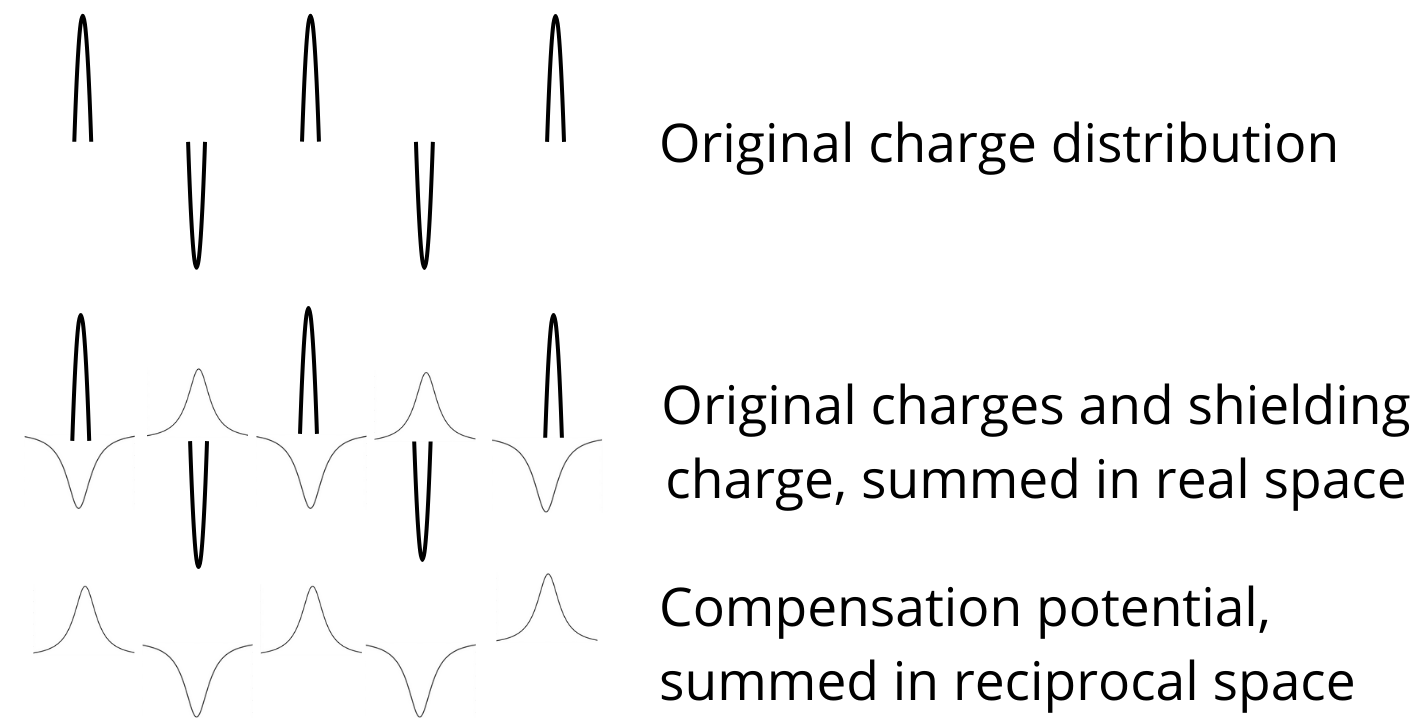
\includegraphics[width=1.0\linewidth]{img/ewald.png} 
	\caption{caption}
	\label{fig:ewald}    
\end{figure} 
\subsubsection{Particle-Particle Particle-Mesh}
Like the Ewald summation method, particle-particle particle-mesh (PPPM) addresses the challenge of accurately modeling interactions between charged particles that extend over long distances while accounting for periodic boundary conditions. PPPM is particularly well-suited for systems with a large number of particles, where the computational cost of traditional methods like Ewald summation becomes prohibitive.

Particle-Particle Interactions: PPPM divides the electrostatic interactions into short-range (particle-particle) and long-range (particle-mesh) components. The short-range interactions involve direct pairwise interactions between particles within a specified cutoff distance. These interactions are computed using standard techniques such as the Coulomb potential or other appropriate force fields.

Particle-Mesh Interactions: The long-range interactions are calculated using a mesh-based approach. PPPM discretizes the charge distribution onto a grid (mesh) using interpolation techniques. The charge density is spread onto the mesh, and then the electric field due to this charge distribution is calculated using Fast Fourier Transform (FFT) techniques.

FFT computation: FFT is used to transform the charge density from real space to reciprocal space (Fourier space), where the long-range interactions can be efficiently computed. In reciprocal space, the electric field due to the charge distribution can be expressed as a convolution between the charge density and the Green's function for the electrostatic potential.

Force calculation: Once the electric field in reciprocal space is computed, it is transformed back to real space using inverse FFT. Then, the forces on particles due to long-range interactions are calculated based on the interpolated electric field at the positions of the particles.

Combining short-range and long-range interactions: The short-range and long-range forces are then combined to obtain the total force acting on each particle in the system. These forces are used to update the positions and velocities of the particles over the course of the simulation.

PPPM offers significant computational advantages compared to direct summation methods, especially for systems with a large number of particles, as it scales more efficiently with system size. However, PPPM requires careful tuning of parameters such as grid spacing and interpolation methods to achieve accurate results. Despite this, PPPM remains a widely used method in MD simulations, enabling researchers to study complex systems with long-range electrostatic interactions efficiently and accurately.


\subsection{Molecular dynamics}
The molecular dynamics method is based on solving the equations of motion of classical Newtonian mechanics for atoms. Let us choose the assumption that the interaction potential $U$ is continuous and differentiable. The force acting on the $i$ particle can thus be written as an equation \ref{sila1} 
\begin{equation}\label{sila1}
	f_i=-\frac{\partial U(r^N)}{\partial r_i}, \qquad i=1,...,N.
\end{equation}

In molecular dynamics, we are focused on the time development of the model. In other words, we are looking for the trajectory of the solution of the respective systems of differential equations. In Newtonian mechanics, acceleration is directly related to forces through the equations of motion. Formally, we can write the equation \ref{sila2}
\begin{equation}\label{sila2}
	\Ddot{r_i}=\frac{f_i}{m_i}, \qquad i=1,...,N,
\end{equation}
where the second time derivative of the positions appears on the left side. The equation \ref{sila2} is a system of 3$N$ ordinary differential equations for a set of $N$ atoms. As initial conditions, we usually choose the knowledge of all atomic positions $r_i$ and velocities $\dot{r_i}$ at the initial time $t=t_0$. 

We solve equation \ref{sila2} using the finite difference method when we track the desired solution in the form of the function $r_i(t), i=1,..,N$, in the time interval $[t_0,t_{max}]$ at discrete points of the form $t=t_0+kh$, where $h$ is the integration step and $k$ is a non-negative integer.

To find a solution, it is necessary to calculate the forces acting on individual particles at each step of the simulation. One of the methods that is applied in this area is the Verlet integration method. It is a simple and very effective method that provides sufficiently accurate results in the physico-chemical context. Its great advantage is the time-reversibility and the conservation of the total energy of the system~\cite{mdskripta}.

\subsubsection{Verlet integration}
Verlet integration method is a numerical method for integrating the equation \ref{sila1}. We express the second derivative using finite differences. From the second-order Taylor expansion $r_i(t\pm h)$ centred at $t$, we obtain the formula
\begin{equation}\label{sila3}
	\Ddot{r_i}=\frac{r_i(t-h)-2r_i(t)+r_i(t+h)}{h^2},
\end{equation}
binding values at three points in a row ($t-h$, $t$ and $t+h$). We will use this characteristic to calculate $r_i(t+h)$. By substituting \ref{sila3} into \ref{sila1} we get 
\begin{equation}\label{sila4}
	r_i(t+h)=2r_i(t)-r_i(t-h)+h^2\frac{f_i(t)}{m_i}.
\end{equation}
In this formulation, we are able to calculate the new positions at time $t+h$ from knowledge of the forces at time $t$, the positions of the particles at time $t$ and the previous time $t-h$. The time reversibility of the method is clearly visible here. The advantage is that the force is calculated only once in each step of the simulation. For the position preceding the initial position ($r_i(t_0-h)$), we can use the expansion \ref{sila5}
\begin{equation}\label{sila5}
	r_i(t_0-h)=r_i(t)-h\dot{r_i}(t_0)+h^2\frac{f_i(t_0)}{2m_i}.
\end{equation}

\subsubsection{Constraint dynamics}

When integrating equations of motion, we often impose constraints on certain aspects of molecular geometries. The main reason is to enable using a longer simulation time step. If we simulate with a too large time step, we introduce large errors into the simulations, leading in extreme cases to a crash of the simulation. The calculated particle positions at time $t+h$ may lead to overlapping of particles, the calculated force acting on the particles may divert from physically reasonable configurations. Conversely, the use of inappropriately short simulation steps reduces the efficiency of the simulations (the most computationally and therefore time consuming element of the simulations is the calculation of the forces when integrating the equations of motion). \cite{mdskripta} The criterion determining the optimal step length is the accuracy of the conservation of total energy. The step length can be determined by an Nyquist-Shannon \cite{shannon_communication_1949} sampling theorem that says that the time step must be half or less of the period of the quickest dynamics exhibited in the system. Thus, for systems containing very light hydrogen atoms, we can either artificially increase the mass of the hydrogen atom while redistributing the masses of the other molecules to conserve the overall mass of the molecule, or fix the bond angles or bond lengths terminating in the hydrogen atoms. It is the fixation of hydrogen bond lengths that is most often implemented in the Verlet method, using an algorithm called SHAKE. 

The SHAKE algorithm is based on Verlet's integration method and is iterative. The first step is to initialize the initial velocities and positions of the atoms, then calculate the positions using Verlet's method without considering bond length constraint. We then create the $\lambda$ correction of the atom positions to constrain the bond length. Fixing the bond length allows us to use a longer time step (we are no longer limited by the motion of very light particles) and, unlike fixing angles, does not introduce large deviations in the simulations.

\subsection{Measuring the properties}
\subsubsection{Statistical ensembles}
MD gives us insight into the total energy of the system, which is naturally conserved in simulations. However, real systems are rarely thermodynamically closed and we often expose the system to external pressure or heat exchange. Thus we speak of different statistical ensembles depending on the conservation of quantities.

As already mentioned, the natural ensemble is the so-called microcanonical ensemble, \textbf{NVE}. Thermodynamically it is an adiabatically izolated and closed system, there is no heat exchange while maintaining the total number of particles, total energy and volume. 

Another ensemble is isothermal closed, or sometimes called the canonical ensemble \textbf{NVT}. As the name implies, the thermodynamic temperature and volume are constant, heat exchange occurs with the thermostat. It is used for applications where we are not interested in pressure or pressure is not definable.

For chemists, the most interesting is the \textbf{NPT} ensemble where temperature and pressure are constant. 

Grandcanonical ensemble $ny$VT, izotermal, open, 

\subsubsection{MSD}
\subsubsection{RDF}

% %%%%%%%%%%%%%%%%%%%%%%%%%%%%%%%%%%%%%%%%%%%%%%%%%%%%%%%%%%%%%%%%%%%%%%%%%
\newpage
\section{COMPUTATIONAL METHODS}

%%%%%%%%%%%%%%%%%%%%%%%%%%%%%%%%%%%%%%%%%%%%%%%%%%%%%%%%%%%%%%%%%%%%%%%%%%%%%%%%%%%%%%%%
%%%%%%%%%%%%%%%%%%%%%%%%%%%%%%%%%%%%%%%%%%%%%%%%%%%%%%%%%%%%%%%%%%%%%%%%%%%%%%%%%%%%%%%%

LAMMPS software \cite{thompson_lammps_2022} (version 5 May 2020) was used for all molecular dynamics calculations. The placement of molecular chains in the simulation boxes was done by Packmol \cite{martinez_p_2009}, the chains were randomly distributed in the space of a cubic box preventing the  overlap. The input files for the LAMMPS software were generated using the fftool \cite{fftool} script written in the Python programming language.

We also used periodic boundary conditions in the directions of all axes and the velocity Verlet integrator. Contributions of long-range charge interactions of distant atoms were calculated using the long-range solver using the particle-particle-particle mesh (PPPM) algorithm \cite{hockney_computer_2021}. The bonds and angles were considered as harmonic oscillators, and for dihedral angles, OPLS (Optimised Potentials for Liquid Simulations) was used for every term.  Coulombic point charges and the Lennard-Jones potential were used to model the particles interaction the cut-off distance for dispersion and Coulombic interactions was set to 12 \r{A}. The SHAKE algorithm \cite{ryckaert_numerical_1977} was applied to constrain the lengths of covalent bonds that terminate in hydrogen atoms. The simulations were run under $NpT$ conditions using the Nosé-Hoover thermostat and barostat \cite{tuckerman_liouville-operator_2006}, with relaxation times for temperature control as 100 fs and pressure control as 1000 fs. The simulations contained around 25~000 atoms in a simulation box. From previous research, this was considered to be a suitable setting. \cite{klajmon_glass_2023}

All-atom non-polarisable force fields were used during MD simulations, the parameterisation of the PLA force field was obtained from the literature \cite{mcaliley_development_2011}, the parameterizations of APIs were also taken from the literature. \cite{cervinka_structure_2021}

\subsection{Simulations of neat PLA}
The PLA was first simulated separately from two initial conformers, a fibrilar and a globular chain. We try to verify that the resulting state of the system does not depend on the initial conformations that were used for the simulations. The Cartesian coordinates of the positions of atoms forming a globule were obtained from the last frame of a simulation of one linear polymer molecule in a large virtual empty box.

The initial simulation of the polymers led to the equilibration of the system. The simulation was carried out at 500 K and 1 bar in three blocks with a gradually increasing simulation step. First with a step 0.2 fs for 0.5 ns, followed by steps 0.4 fs and 0.7 fs each for 0.7 ns, then 1 ns of simulation with step a 1 fs. 





\subsection{Simulations of neat APIs and mixtures with PLA}
We started all simulations with an equilibration simulation run from randomly packed simulation boxes under the temperature of 500~K and pressure of 1 bar in three blocks with a gradually increasing time-integration step. The simulation began with an equilibration procedure using a step of 0.25~fs, followed by steps 0.5 and 0.75~fs each for a simulation time of 0.5~ns, then 1~ns of simulation with a step of 1~fs. From this point, we cooled the system, down to 300~K over 2~ns with a step of 1~fs. After this cooling, we continued with a 10~ns long production run with a temperature of 300~K and pressure equal to 1~bar.

From these production runs, we evaluated the MSD (Mean Squared Displacement) of API and PLA molecules in the mixture and the RDF (radial distribution function) of atom interactions. We also performed a production run at the higher temperature of 500~K and the same pressure of 1 bar starting from conformations after the first equilibration under 500~K. We also sampled RDFs and MSDs. Those simulations were performed for neat APIs, PLA polymer, and mixtures with different concentrations of API. For each API, the concentration ratio API:PLA in terms of the number of molecules in a simulation box was 100:17, 200:17, and 300:17. The corresponding molar and mass fractions are available in the Table \ref{tab:fractions}.

\begin{table}[h]
	\centering
	\caption{The concentration of API in mixtures with PLA, expressed in molar and mass fractions.}
	\begin{tabular}{ccccccc}
		\toprule
		{\textbf{\boldmath{$N_{\text{API}}$}}} &
		{\textbf{\boldmath{$N_{\text{PLA}}$}}} &
		{\textbf{\boldmath{$x_{\text{API}}$}}} & {\textbf{\boldmath{$w_{\text{nap}}$}}} & {\textbf{\boldmath{$w_{\text{cbz}}$}}} & {\textbf{\boldmath{$w_{\text{ibu}}$}}} & {\textbf{\boldmath{$w_{\text{indo}}$}}} \\
		\midrule
		100 & 17 & 0.85 & 0.086 & 0.088 & 0.078 & 0.13 \\
		200 & 17 & 0.92 & 0.16 & 0.16 & 0.14 & 0.23 \\
		300 & 17 & 0.95 & 0.22 & 0.22 & 0.20 & 0.30 \\
		\bottomrule
	\end{tabular}
	\label{tab:fractions}
\end{table} 

To determine the glass transition temperature ($T_\mathrm{g}$) of the mixtures, we performed simulated annealing simulations with a gradually decreasing temperature cooling rate (30 K$\ $ ns$^{-1}$) starting at 800~K and ending at 200~K. Systems containing a mixture of API and PLA were first heated from 500~K to 800~K over 2~ns. To have statistically more reliable data, simulated annealing simulations were performed from 5 different initial conformations. To obtain those conformations a 5~ns long simulation at 800~K was done sampling atomic coordinates within the image of the box every 1~ns.  

% %%%%%%%%%%%%%%%%%%%%%%%%%%%%%%%%%%%%%%%%%%%%%%%%%%%%%%%%%%%%%%%%%%%%%%%%%
\newpage
\section{RESULTS AND DISCUSSION}

%%%%%%%%%%%%%%%%%%%%%%%%%%%%%%%%%%%%%%%%%%%%%%%%%%%%%%%%%%%%%%%%%%%%%%%%%%%%%%%%%%%%%%%%
%%%%%%%%%%%%%%%%%%%%%%%%%%%%%%%%%%%%%%%%%%%%%%%%%%%%%%%%%%%%%%%%%%%%%%%%%%%%%%%%%%%%%%%%

text

% %%%%%%%%%%%%%%%%%%%%%%%%%%%%%%%%%%%%%%%%%%%%%%%%%%%%%%%%%%%%%%%%%%%%%%%%%
\clearpage
\section{CONCLUSION}
\
%%%%%%%%%%%%%%%%%%%%%%%%%%%%%%%%%%%%%%%%%%%%%%%%%%%%%%%%%%%%%%%%%%%%%%%%%%%%%%%%%%%%%%%%
%%%%%%%%%%%%%%%%%%%%%%%%%%%%%%%%%%%%%%%%%%%%%%%%%%%%%%%%%%%%%%%%%%%%%%%%%%%%%%%%%%%%%%%%

Methods of computational chemistry were used to study the structural and thermodynamical properties of one representative biocompatible polymer (PLA) and four selected APIs. At fisrt, all studied materials were studied separately as neat substances. Then the properties of amorphous mixtures were determined with regard to interactions of their components at the microscale to establish an interpretation of their macroscopic behavior. 

The glass transition temperature of polylactic acid was determined using molecular dynamics methods and validated by comparison with experimental data. Same validation was done also for densities. The computed values of glass transition temperatures were overestimated compared to their experimental values. It would be beneficial to use a polarizable force field adding explicit polarization to the simulation, this is a part of further research.  

Secondly, binary mixtures of the four selected API with polylactic acid were studied focusing on their intermolecular interactions, mainly the potential hydrogen bonding. Mean-squared displacement and radial distribution functions of the mixtures and neat API were discussed. Series of molecular-dynamics simulations were performed in order to predict the glass-transition temperature of the mixtures. We found that the glass transition temperature for binary mixtures for 3 out of the 4 selected active pharmaceutical ingredients (ibuprofen, indomethacin and naproxen) increased compared to the values for the neat substances. This is consistent with the observation that these APIs exhibited sufficiently strong interactions with the polymer excipient. Those results propose that the addition of the polylactic acid had a beneficial impact on the drug stabilization by forming the amorphous mixture. In contrast, in the case of carbamazepine, the interactions were not sufficient to stabilize the API with the polymer and the mixture did not show an increase in the glass transition temperature. 


% %%%%%%%%%%%%%%%%%%%%%%%%%%%%%%%%%%%%%%%%%%%%%%%%%%%%%%%%%%%%%%%%%%%%%%%%%
% REFERENCES, List of Abbreviations, List of Symbols, List of Tables, 
% List of Figures
% %%%%%%%%%%%%%%%%%%%%%%%%%%%%%%%%%%%%%%%%%%%%%%%%%%%%%%%%%%%%%%%%%%%%%%%%%
% REFERENCES

\newpage
\addcontentsline{toc}{section}{REFERENCES}
% \renewcommand{\refname}{REFERENCE} %changes name of reference section
\bibliography{references} 


% %%%%%%%%%%%%%%%%%%%%%%%%%%%%%%%%%%%%%%%%%%%%%%%%%%%%%%%%%%%%%%%%%%%%%%%%%
% List of Abbreviations

%\newpage
%\addcontentsline{toc}{section}{List of Abbreviations}
%\section*{List of Abbreviations}
%
%\begin{tabular}{ll}
%$x$ & position\\
%$v$ & velocity\\
%...\\
%\end{tabular}

% %%%%%%%%%%%%%%%%%%%%%%%%%%%%%%%%%%%%%%%%%%%%%%%%%%%%%%%%%%%%%%%%%%%%%%%%%
% List of Symbols

%\newpage
%\addcontentsline{toc}{section}{List of Symbols}
%\section*{List of Symbols}
%
%\begin{tabular}{ll}
%$x$ & position\\
%$v$ & velocity\\
%...\\
%\end{tabular}

% %%%%%%%%%%%%%%%%%%%%%%%%%%%%%%%%%%%%%%%%%%%%%%%%%%%%%%%%%%%%%%%%%%%%%%%%%
% List of Tables

%\newpage
%\addcontentsline{toc}{section}{List of Tables}
%\section*{List of Tables}
%\listoftables

% %%%%%%%%%%%%%%%%%%%%%%%%%%%%%%%%%%%%%%%%%%%%%%%%%%%%%%%%%%%%%%%%%%%%%%%%%
% List of Figures

%\newpage
%\addcontentsline{toc}{section}{List of Figures}
%\section*{List of Figures}
%\listoffigures



% %%%%%%%%%%%%%%%%%%%%%%%%%%%%%%%%%%%%%%%%%%%%%%%%%%%%%%%%%%%%%%%%%%%%%%%%%
% Appendix
% %%%%%%%%%%%%%%%%%%%%%%%%%%%%%%%%%%%%%%%%%%%%%%%%%%%%%%%%%%%%%%%%%%%%%%%%%
% Appendix

\newpage

\appendix
\begin{appendices}
% %%%%%%%%%%%%%%%%%%%%%%%%%%%%%%%%%%%%%%%%%%%%%%%%%%%%%%%%%%%%%%%%%%%%%%%%%
\section{Headline}

\end{appendices}

	
% %%%%%%%%%%%%%%%%%%%%%%%%%%%%%%%%%%%%%%%%%%%%%%%%%%%%%%%%%%%%%%%%%%%%%%%%%
\end{document}
